%%%%%%%%%%%%%%%%%%%%%%%%%%%%%%%%%%%%%%%%%%%%%%%%%%%%%%%%%%%%%%%%%%%%%%%%%%%%

% It may help to know that the lecture on homotopy was given on Feb. 14th

%%%%%%%%%%%%%%%%%%%%%%%%%%%%%%%%%%%%%%%%%%%%%%%%%%%%%%%%%%%%%%%%%%%%%%%%%%%%


\documentclass{notes}

\usepackage{makeidx}

\makeindex

\theoremstyle{plain}
\newtheorem{proposition}{Proposition}[chapter]
\newtheorem{theorem}[proposition]{Theorem}
\newtheorem{corollary}[proposition]{Corollary}
\newtheorem{definition}[proposition]{Definition}
\newtheorem{lemma}[proposition]{Lemma}
\newtheorem*{example}{Example}
\newtheorem*{examples}{Examples}
\newtheorem*{notes}{N.B}
\newtheorem*{notation}{Notation}
\newtheorem*{remark}{Remark}

\newcommand{\Cinf}{\C_\infty}
\newcommand{\T}{\mathbb{T}}
\newcommand{\cU}{\mathcal{U}}
\newcommand{\cV}{\mathcal{V}}
\newcommand{\cN}{\mathcal{N}}
\newcommand{\quot}[1]{#1/\negthickspace\sim\,}

\DeclareMathOperator{\inter}{int}
\DeclareMathOperator{\Res}{Res}
\DeclareMathOperator{\ord}{ord}

% If you like symbolic footnotes, uncomment next line.

% \renewcommand{\thefootnote}{\ensuremath{\fnsymbol{footnote}}}

\begin{document}
\frontmatter
\title{Further Analysis}

\lecturer{Prof.~W.T.~Gowers}
\maintainer{Paul Metcalfe}
\date{Lent 1997}
\maketitle

\thispagestyle{empty}

\noindent\verb$Revision: 2.8 $\hfill\\
\noindent\verb$Date: 1999/10/22 11:33:59 $\hfill\

\vspace{1.5in}

The following people have maintained these notes.

\begin{center}
\begin{tabular}{ r  l}
-- date & Paul Metcalfe
\end{tabular}
\end{center}

\tableofcontents

\chapter{Introduction}

These notes are based on the course ``Further Analysis''
given by Prof.~W.T.~Gowers%
\footnote{Yes, \emph{that} Prof. Gowers.}
in Cambridge in the Lent Term 1997.  These
typeset notes are totally unconnected with Prof.~Gowers.

\alsoavailable
\archimcopyright

\mainmatter

\chapter{Topological Spaces}

\section{Introduction}

\begin{definition}
  A topological space\index{topological space} is a set $X$ together
  with a collection $\tau$ of subsets of $X$ satisfying the following
  axioms.

\begin{enumerate}
\item $\emptyset, X \in \tau$;
\item If $U_1, \dots, U_n \in \tau$, then $U_1 \cap \dots \cap U_n \in
  \tau$; (that is, $\tau$ is closed under finite intersections)
\item Any union of sets in $\tau$ is in $\tau$ (or $\tau$ is closed
  under any unions).
\end{enumerate}
\end{definition}

\begin{definition}
  $\tau$ is called a topology\index{topology} on $X$.  The sets in
  $\tau$ are
called open sets\index{open sets}.  A subset of $X$ is closed%
\index{closed sets} if its complement is open.
\end{definition}

\begin{examples}
\begin{enumerate}
\item If $(X,d)$ is a metric space and $\tau$ the collection of open
  sets (in a metric space sense) then $(X,\tau)$ is a topological
  space.
\item If $X$ is any set and $\tau$ is the power set of $X$, $(X,\tau)$
  is a
topological space.  $\tau$ is called the discrete topology%
\index{topology!discrete} on $X$.
\item If $X$ is any set and $\tau = \{ \emptyset, X \}$, $(X,\tau)$ is
  a
topological space.  $\tau$ is called the indiscrete topology%
\index{topology!indiscrete} on $X$.
\item If $X$ is any infinite set, and $\tau = \{ Y \subset X: X
  \setminus Y \text{ is finite}\} \cup \{\emptyset\}$ then $(X,\tau)$
  is a topological space.
$\tau$ is called the cofinite topology%
\index{topology!cofinite} on $X$.
\item If $X$ is any uncountable set, and $\tau = \{ Y \subset X: X
  \setminus Y \text{ is countable}\} \cup \{\emptyset\}$ then
  $(X,\tau)$ is a topological
space.  $\tau$ is called the cocountable topology%
\index{topology!cocountable} on $X$.
\end{enumerate}
\end{examples}

\begin{definition}
Let $A$ be a subset of a topological space.  The closure%
\index{closure} of $A$, % 
denoted $\overline{A}$, is the intersection of all closed sets
containing $A$.  Note that $\overline{A}$ is closed and any closed set
containing $A$ contains $\overline{A}$.
\end{definition}

\begin{definition}
Let $A$ be a subset of a topological space.  The interior%
\index{interior} of $A$, denoted $\inter A$ or $A^0$ is the union of
all open sets in $A$.  Note that $\inter A$ is open and any open set
in $A$ is in $\inter A$.
\end{definition}

\begin{definition}
  The boundary\index{boundary} $\partial A$ of a set A is
  $\overline{A} \setminus \inter A$.
\end{definition}

\begin{definition}
  Let $(x_n)_1^\infty$ be a sequence in a topological space
  $(X,\tau)$.  We say that $x_n$ converges to $x$ ($x_n \rightarrow
  x$) if for every open set $U$ such that $x \in U$, $\exists\ N$ such
  that $n \ge N \Rightarrow x_n \in U$.  This agrees with the usual
  definition for metric spaces.
\end{definition}

\begin{definition}
  Let $(X,\tau)$ and $(Y,\sigma)$ be topological spaces and let $f
  \colon X \mapsto Y$.  We say that $f$ is continuous if for every $U
  \in \sigma$, $f^{-1}(U) \in \tau$.  (Or inverse image of an open set
  is open.)
\end{definition}

It follows from results in Analysis that this definition agrees with
the usual $\epsilon - \delta$ definition if $X$ and $Y$ are metric
spaces.

\begin{definition}
Let $(X,\tau)$ be a topological space and let $x \in X$.  A neighbourhood%
\index{neighbourhood} of $x$ is a set $N$ that contains an open set
containing $x$.
\end{definition}

\begin{proposition}
  Let $(X,\tau)$ and $(Y,\sigma)$ be topological spaces and let $f
  \colon X \mapsto Y$.  Then the following are equivalent :-
\begin{enumerate}
\item $f$ is continuous.
\item For every $x \in X$ and every neighbourhood $M$ of $f(x)$ there
  exists a neighbourhood $N$ of $x$ such that $f(N) \subset M$.
\end{enumerate}
\end{proposition}

\begin{proof}
  Firstly do $1 \Rightarrow 2$.  $M$ contains an open set $U$
  containing $f(x)$.  Then $N = f^{-1}(U)$ is a neighbourhood of $x$
  such that $f(N) \subset U$.
  
  Now do the case $2 \Rightarrow 1$.  Let $U$ be an open subset of
  $Y$. For every $x \in f^{-1}(U)$, $U$ is a neighbourhood of $f(x)$.
  We can find a neighbourhood $N_x$ of $x$ such that $f(N_x) \subset
  U$.  Now $N_x$ contains an open set $V_x$ containing $x$.  Let
\[
V = \bigcup_{x \in f^{-1}(U)} V_x.
\]
Then $f(V_x) \subset U \; \forall x$, so $f(V) \subset U$ and $V
\subset f^{-1}(U)$.  But $V \supset f^{-1}(U)$ so $V = f^{-1}(U)$.
$V$ is open, so $f^{-1}(U)$ is open and $f$ is continuous.
\end{proof}

\begin{definition}
  Let $(X,\tau)$ and $(Y,\sigma)$ be topological spaces and $f \colon
  X \mapsto Y$.
$f$ is a homeomorphism\index{homeomorphism} %
if it is continuous with a continuous inverse.
\end{definition}

\begin{example}
  $\R$ and $(0,1)$ with usual metrics are homeomorphic.
\end{example}

\section{Building New Spaces}

\begin{definition}
Let $(X,\tau)$ be a topological space and $Y \subset X$.  The subspace
topology\index{topology!subspace} on $Y$ is 
\[
\{ U \cap Y : U \in \tau \}.
\]
\end{definition}

\begin{proposition}
Let $(X,d)$ be a metric space, $Y \subset X$ and $U \subset Y$.  Then the
following are equivalent.
\begin{enumerate}
\item $U$ is open in the subspace topology on $Y$.
\item For every $u \in U, \exists\ \delta > 0$ such that if $v \in Y, d(u,v)
< \delta$ then $v \in U$.
\end{enumerate}
\end{proposition}

\begin{proof}
Do $1 \Rightarrow 2$.  Let $u \in U$.  Since $U$ open in $Y$, $\exists\ V
\subset X$, $V$ open such that $U = V \cap Y$.  Then $\exists\ \delta > 0$
such that $d(u,v) < \delta \Rightarrow v \in V$.  Now $d(u,v) < \delta$
and $v \in Y \Rightarrow v \in V \cap Y = U$.

Now do $2 \Rightarrow 1$.  Suppose $U$ satisfies 2.  For every $u \in U$,
pick $\delta = \delta(u) > 0$ such that $d(u,v) < \delta$ and $v \in Y
\Rightarrow v \in U$.  Let $N_u = \{v \in X : d(u,v) < \delta \}$.  Now
$N_u$ is open and $V = \bigcup_{u \in U} N_u$ is open.  Now $V \cap Y = U$.
\end{proof}

\begin{definition}
Let $(X,\tau)$ be a topological space and $\sim$ be an equivalence relation on
$X$.  Denote the set $\quot{X}$ by $Y$ and let $q \colon X \mapsto Y$ be the
equivalence map. (ie if $x \in X$, $q(x)$ is the equivalence class of $x$).
The quotient topology\index{topology!quotient} on $Y$ is
$\{ U \in Y : q^{-1}(U) \in \tau\}$.
\end{definition}

\begin{notes}
\begin{enumerate}
\item $q^{-1}(U)$ is the union of the equivalence classes in U.
\item Notice $q$ is continuous and that the quotient topology is the
largest topology making it so.
\end{enumerate}
\end{notes}

\begin{examples}
\begin{enumerate}
\item Let $\tau$ be the usual topology on $\R$.  Then the subspace topology
on $\Z \subset \R$ coincides with the discrete topology on $\Z$.
\item Let $\tau$ be as in 1.  Then the interval $(\frac{1}{2},1]$ is open
in the subspace topology on $[0,1]$.
\item Let $\sim$ be the equivalence relation on $\R$ defined by $x \sim y
\Leftrightarrow x-y \in \Z$.  Let $[x]$ denote the equivalence class
of $x$.  Then the map \[
\phi \colon \quot{\R} \mapsto \T \equiv \{ z \in \C : 
\abs{z}=1 \}
\] is both well defined and a homeomorphism.
\end{enumerate}
\end{examples}

\begin{definition}
Let $(X,\tau)$ and $(Y,\sigma)$ be topological spaces. The product topology%
\index{topology!product} %
on $X \times Y$ is the collection of all possible unions of sets of the form
$U \times V$ with $U \in \tau$ and $V \in \sigma$.  Similarly, if 
$(X_i,\tau_i)_{i=1}^{n}$ are $n$ topological spaces, the product topology 
on $\prod_{i=1}^n X_i$ is the collection of all unions of sets 
$\prod_{i=1}^n U_i$ with $U_i \in \tau_i$.
\end{definition}

\begin{example}
If $\R$ has its usual topology, then the product topology on $\R \times \R$
is the same as the usual topology on $\R \times \R \equiv \R^2$.
\end{example}

\begin{proof}
Let us write $\pi$ for the product topology on $\R \times \R$ and $\sigma$ for
the usual (Euclidean) topology.  Let $U \in \sigma$.  Then given $(x_1,x_2) \in
U$, $\exists\ \delta > 0$ such that $d((x_1,x_2),(y_1,y_2))<\delta
\Rightarrow (y_1,y_2) \in U$.  Then the $\pi$-open set
$(x-\frac{\delta}{2},x+\frac{\delta}{2}) \times 
(x-\frac{\delta}{2},x+\frac{\delta}{2}) \subset U$ and contains $(x_1,x_2)$,
so $U$ is $\pi$-open, given $\sigma \subset \pi$.  Conversely, every set of
the form $A \times B$ with $A,B$ open in $\R$ is open in $\R^2$.  The union
of such sets is $\sigma$-open, giving $\pi \subset \sigma$ and $\pi = \sigma$.
\end{proof}

Exercise to show that $X \times (Y \times Z) = X \times Y \times Z$ as
topological spaces.

\begin{definition}
Let $(X,\tau)$ be a topological space.  A basis%
\index{basis} for $\tau$ (or a basis of
open sets) is a subset $\beta \subset \tau$ such that every $U \in \tau$ is
a union of sets in $\beta$.  The sets in $\beta$ are called basic open sets.
If $x \in X$, then a basis of neighbourhoods%
\index{neighbourhood!basis of neighbourhoods} of $x$ is a collection $\cN$ of
neighbourhoods of $x$ such that every neighbourhood of $x$ contains
$N \in \cN$.
\end{definition}

\begin{examples}
\item The sets $U \times V$ with $U \in \tau$ and $V \in \sigma$ are a basis
for the product topology on $(X,\tau) \times (Y,\sigma)$.
\item The sets $\{y : d(x,y) \le \frac{1}{n}\}$ are a basis of neighbourhoods
for a point $x$ in a metric space.
\end{examples}

\begin{proposition}
The quotient topology and product topology are topologies.
\end{proposition}

\begin{proof}
The result for the quotient topology follows easily from the fact that $q^{-1}$
preserves unions and intersections.  For products let $(X_i,\tau_u)_{i=1}^n$
be topological spaces. Everything is simple except closure under finite
intersections.  By induction it is sufficient to prove for two sets.

If $U_i \in \tau_i$, call $U_1 \times \dots \times U_n$ an
{open box}\footnote{This is not standard terminology.}.  Firstly, observe
that
\[
\left(
U_1 \times \dots \times U_n
\right)
\cap
\left(
V_1 \times \dots \times V_n
\right)
=
\left(
U_1 \cap V_1
\right)
\times
\dots
\times
\left(
U_n \cap V_n
\right)
\]
and thus the intersection of two open boxes is an open box.  Now take
\[
\bigcup_{\gamma \in \Gamma} B_\gamma \text{ and } 
\bigcup_{\delta \in \Delta} C_\delta, 
\]
with all $B_\gamma$'s and $C_\delta$'s open boxes.

Now
\[
\bigcup_{\gamma \in \Gamma} B_\gamma \cap 
\bigcup_{\delta \in \Delta} C_\delta = \bigcup_{\substack{\gamma \in \Gamma \\
\delta \in \Delta}}
B_\gamma \cap C_\delta,
\] which is a union of open boxes, and so open.
\end{proof}

\chapter{Compactness}

\section{Introduction}

\begin{definition}
Let $(X,\tau)$ be a topological space.  An open cover%
\index{open cover} of $X$ is a collection
$\{U_\gamma : \gamma \in \Gamma\}$ of open sets such that
$X = \bigcup_{\gamma \in \Gamma} U_\gamma$.  If $Y \subset X$ then 
an open cover of $Y$ is a collection $\{ U_\gamma : \gamma \in \Gamma\}$
such that $Y \subset \bigcup_{\gamma \in \Gamma} U_\gamma$.

A subcover of a cover $\cU = \{ U_\gamma : \gamma \in \Gamma \}$ is a subset
$\cV \subset \cU$ which is still an open cover.
\end{definition}

\begin{examples}
\begin{enumerate}
\item $\{I_n = (-n,n), n = 1, 2, \dots\}$ is an open cover for $\R$.
$\{ I_{n^2} \}$ is a subcover.
\item The intervals $I_n = (n-1,n+1)$ with $n \in \Z$ form a cover of the reals
with no proper subcover.
\end{enumerate}
\end{examples}

\begin{definition}
A topological space $(X,\tau)$ is compact\index{topological space!compact} %
if every open cover has a finite subcover.
\end{definition}

\begin{examples}
The open covers mentioned above show that $\R$ is not compact.  Any finite
topological space is compact, as is any set with the indiscrete topology.
\end{examples}

\section{Some compact sets}

\begin{lemma}
Let $(X,\tau)$ be a topological space with $Y \subset X$.  Then the following
are equivalent :-
\begin{enumerate}
\item $Y$ is compact in the subspace topology.
\item Every cover of $Y$ by $U_\gamma \in \tau$ has a finite subcover.
\end{enumerate}
\end{lemma}

\begin{proof}
$1 \Rightarrow 2$.  Let $Y \subset \bigcup_{\gamma \in \Gamma} U_\gamma$ with
$U_\gamma \in \tau$.  Then $Y = \bigcup_{\gamma \in \Gamma} (U_\gamma \cap Y)$
with $U_\gamma$ open in $Y$.  Since $Y$ is compact $\exists\ \gamma_1, \dots
, \gamma_n$ such that $Y = \bigcup_{i=1}^n (U_{\gamma_i}\cap Y)$, which gives
that $Y \subset \bigcup_{i=1}^n U_{\gamma_i}$.

$2 \Rightarrow 1$.  Let $Y = \bigcup_{\gamma \in \Gamma} V_\gamma$ with
$V_\gamma$ open in $Y$.  Since $V_\gamma = U_\gamma \cap Y$ for some $U_\gamma$
open in X, $Y \subset \bigcup_{\gamma \in \Gamma}U_\gamma$.  By assumption,
$\exists\ \gamma_1, \dots, \gamma_n$ such that
$Y \subset \bigcup_{i=1}^{n}U_{\gamma_i}$.  This implies that
$Y = \bigcup_{i=1}^n (U_{\gamma_i}\cap Y) = \bigcup_{i=1}^n V_{\gamma_i}$.
\end{proof}

\begin{theorem}[The Heine-Borel Theorem]\index{Heine-Borel Theorem}
The closed interval $[a,b] \subset \R$ is compact.
\end{theorem}

\begin{proof}
Let $[a,b] \subset \bigcup_{\gamma \in \Gamma} U_\gamma$ with $U_\gamma$ open
in $\R$ and let
\[
K = \{ x \in [a,b] : [a,x] \text{ is contained in a finite
union of open sets}\}.
\]
Let $r = \sup K$. Then $r \in [a,b]$, so $r \in U_\gamma$ for some $\gamma$.
But $U_\gamma$ is open, so $\exists\ \delta >0$ such that
$[r-\delta,r+\delta] \subset U_\gamma$.  By the definition of $r$,
$[a,r-\delta]$ has a finite open cover, thus $[a,r+\delta]$ has a finite
open cover.  This is a contradiction, unless $r = b$.
\end{proof}

\begin{theorem}
A continuous image of a compact set is compact.
\end{theorem}

\begin{proof}
Let $X$ be compact and let $f \colon X \mapsto Y$ be continuous.  Now
$f(X) \subset \bigcup_{\gamma \in \Gamma} U_\gamma$ with $U_\gamma$ open in
$Y$.  Since $f$ is continuous, $f^{-1}(U_\gamma)$ is open in $X\ \forall\ 
\gamma \in \Gamma$ and furthermore $X = \bigcup_{\gamma \in \Gamma} f^{-1}
(U_\gamma)$.  Since $X$ is compact, $\exists\ \gamma_1, \dots, \gamma_n$
such that $X = \bigcup_{i=1}^n f^{-1}(U_{\gamma_i})$.  Thus $f(X) \subset
\bigcup_{i=1}^n U_{\gamma_i}$.
\end{proof}

\begin{theorem}
A closed subset of a compact set is compact.
\end{theorem}

\begin{proof}
Let $X$ be compact and $K \subset X$ be closed.  Let $K \subset
\bigcup_{\gamma \in \Gamma} U_\gamma$ with $U_\gamma$ open in $X$.  Now
$X = (X \setminus K) \cup \left( \bigcup_{\gamma \in \Gamma} U_\gamma \right)$.
Since $X$ is compact, $\exists$ a finite subcover and 
$X = (X \setminus K) \cup \left( \bigcup_{i=1}^n U_{\gamma_i} \right)$.  Then
$K \subset \bigcup_{i=1}^n U_{\gamma_i}$.
\end{proof}

\begin{definition}
A topological space $(X,\tau)$ is called Hausdorff%
\index{topological space!Hausdorff}, if given any two distinct
$x,y \in X$, there exist disjoint open sets $U$ and $V$ with $x \in U$ and
$y \in V$.
\end{definition}

\begin{examples}
\begin{enumerate}
\item Any metric space is Hausdorff.  Given $x,y$ distinct, let
$U = \{ z : d(x,z) < d(x,y)/2\}$ and $V = \{ z : d(y,z) < d(x,y)/2\}$.
\item Any set with more than one element and the indiscrete topology is
not Hausdorff.
\end{enumerate}
\end{examples}

\begin{theorem}
Every compact subset of a Hausdorff topological space is closed.
\end{theorem}

\begin{proof}
Let $X$ be Hausdorff and $K \subset X$ be compact.  If $x \notin K$ and
$y \in K$ then one can find disjoint open sets $U_{xy}$ and $V_{xy}$ with
$x \in U_{xy}$ and $y \in V_{xy}$.  For fixed $x$, the sets $V_{xy}, y \in
K$ form an open cover of $K$.  Hence $\exists\ y_1, \dots, y_n$ such that
$K \subset \bigcup_{i=1}^n V_{xy_i}$  Let $U_x = \bigcap_{i=1}^n U_{xy_i}$
and $V_x = \bigcup_{i=1}^n V_{xy_i}$.  Note that $U_x \cap V_x = \emptyset$,
$x \in U_x$, $K \subset V_x$ and $U_x \cap K = \emptyset$.  But
$\bigcup_{x \notin K} U_x = X \setminus K$ is open.
\end{proof}

\begin{theorem}
A product of finitely many compact sets is compact.
\end{theorem}

\begin{proof}
It is enough to do two sets.  The general result follows by induction 
(and $X \times (Y \times Z) = X \times Y \times Z$).

Let $X$ and $Y$ be compact and let $X \times Y = \bigcup_{\gamma \in \Gamma}
U_\gamma$, $U_\gamma$ open in $X \times Y$.  $U_\gamma$ is the union of sets
of the form $V \times W$, with $V$ open in $X$ and $W$ open in $Y$.  It
follows that $X \times Y = \bigcup_{\delta \in \Delta} V_\delta \times 
W_\delta$ with $V_\delta$ open in $X$ and $W_\delta$ open in $Y$,
$V_\delta \times W_\delta \subset U_\gamma$.  Let $x \in X$.  Now
\[
\{ x \} \times Y 
\subset 
\bigcup_{\substack{\delta \in \Delta \\ x \in V_\delta}} V_\delta \times
W_\delta.
\]
Since $Y$ is compact, one can find $\delta_1, \dots, \delta_n$ such that
$Y = \bigcup_{i=1}^n W_{\delta_i}$.  Let $V_x = \bigcap_{i=1}^n V_{\delta_i}$.
The sets $V_x$ form an open cover of $X$, thus $\exists\ x_1, \dots, x_n$
such than $X = \bigcup_{j=1}^m V_{x_j}$.  Now $X \times Y = \bigcup_{j=1}^m
V_{x_j} \times Y$.  But $V_{x_j} \times Y$ has a finite cover of $(V_\delta
\times W_\delta)$'s.  For each $V_\delta \times W_\delta$, choose $U_\gamma$
with $V_\delta \times W_\delta \subset U_\gamma$ to obtain a finite open
cover of $X \times Y$. 
\end{proof}

\begin{theorem}
A subset of $\R^n$ is compact iff it is closed and bounded.
\end{theorem}

\begin{proof}
Let $X \subset \R^n$ be closed and bounded.  Then $\exists\ M$ such that
$d(x,0) \le M \forall\ x \in X$.  In particular, $X \subset [-M,M]^n$. But
$[-M,M]$ is compact, so $[-M,M]^n$ is compact.  But $X$ is closed, so $X$ is
compact.

Conversely, if $X$ is compact then $X$ is closed, since $\R^n$ is Hausdorff.
If $X$ is not bounded, then the sets $U_m = \{ x \in X : d(x,0) < m \}$ form
an open cover with no finite subcover.
\end{proof}

\section{Consequences of compactness}

\begin{theorem}
A continuous real function on a compact metric space is bounded and
attains its bounds.
\end{theorem}

\begin{proof}
The image of such a function is compact, and so closed and bounded.  Closed
$\Rightarrow$ the function attains its bounds.
\end{proof}

\begin{theorem}
Let $X$ be a compact metric space, let $Y$ be a metric space and let
$f \colon X \mapsto Y$ be continuous.  Then $f$ is uniformly continuous.
\end{theorem}

\begin{proof}
Let $\epsilon > 0$ be arbitrary.  We must show $\exists\ \delta > 0\ 
\forall\ x,y \in X d(x,y) < \delta \Rightarrow d(f(x),f(y)) < \epsilon$.
Since $f$ is continuous, $\forall\ x \in X\  \exists\ \delta_x > 0\ \forall\ y
\in X d(x,y) < 2 \delta_x \Rightarrow d(f(x),f(y)) < \epsilon/2$.

Now let $U_x = \{ y : d(x,y) < \delta_x \}$.  Then the $U_x$ form an open cover
of $X$, so $\exists\ x_1, \dots, x_n$ such that
$X = \bigcup_{i=1}^n U_{x_i}$.  Let $\delta = \min \delta_{x_i}$.

Let $d(y,z) < \delta$.  Since the $U_{x_i}$ form a cover we can find $i$ such
that $d(x_i,y) < \delta_{x_i}$ and $d(x_i,z) < \delta_{x_i}$.  By the
definition of the $U_{x_i}$, $d(f(y),f(z)) < \epsilon$ by the triangle
inequality.
\end{proof}

\begin{lemma}
Let $X$ be a metric space and let $K \subset X$ be compact and $Y \subset X$
be closed.  Then $\exists\ x \in K$ such that $d(x,Y) = \inf \{ d(x,w) :
x \in K, w \in Y \}$.
\end{lemma}

\begin{proof}
Define $f \colon K \mapsto \R$ by $f(x) = dist(x,Y)$.  This is continuous, and so
attains its lower bound.
\end{proof}

In particular, if $K$ and $Y$ are disjoint, then $d(x,Y) > 0$ for every $x$
as $Y$ is closed. Hence $\exists\ \delta > 0$ such that $d(x,Y) \ge \delta\
\forall\ x \in X$.

\section{Other forms of compactness}

\begin{definition}
$X$ is sequentially compact\index{topological space!sequentially compact}
if every sequence in $X$ has a convergent subsequence.
\end{definition}

Bolzano-Weierstrass is the statement that a closed bounded subset of $\R^n$
is sequentially compact.

\begin{theorem}
A compact metric space is sequentially compact.
\end{theorem}

\begin{proof}
Let $X$ be a metric space and let $(x_n)_1^\infty$ be a sequence with no
convergent subsequence.

Now, claim that $\forall\ x \in X\ \exists\ \delta > 0$ such that
$d(x,x_n) < \delta$ for at most finitely many $n$.  Otherwise $\exists\ x$
such that $d(x,x_n) < m^{-1}$ infinitely many times.  Now easy to construct
a convergent subsequence.

For each $x$, pick such a $\delta$ and let $U_x = \{y : d(x,y) < \delta \}$.
The $U_x$ thus form an open cover with no finite subcover.
\end{proof}

\begin{theorem}
Let $X \subset \R^n$.  Then the following are equivalent.
\begin{enumerate}
\item $X$ is compact.
\item $X$ is sequentially compact.
\item $X$ is closed and bounded.
\end{enumerate}
\end{theorem}

\begin{proof}
We know $3 \Leftrightarrow 1 \Rightarrow 2$ from previous theorems.  Thus
enough to show that $2 \Rightarrow 3$.

If $X$ is not closed, $\exists\ x \notin X$ such that $\forall\ m \
\exists\ y_m \in X$ such that $d(y_m,x) < n^{-1}$.  Then every subsequence
of $y_n$ converges in $\R^n$ to $x$ and does not converge in $X$.  If $X$ is
not bounded then $\forall\ n\  \exists\ x_n$ such that $d(0,x_n) \ge n$,
a sequence with no convergent subsequence.
\end{proof}

\chapter{Connectedness}

\section{Introduction}

\begin{definition}
Let $X$ be a topological space.  Suppose $U$, $V \subset X$ such that
\begin{enumerate}
\item $U$, $V$ open,
\item $U \cap V = \emptyset$,
\item $X = U \cup V$,
\item both $U$ and $V$ are non-empty.
\end{enumerate}
Then $U$, $V$ are said to disconnect $X$.  $X$ is connected%
\index{topological space!connected} if no two subsets disconnect $X$.
\end{definition}

If $Y$ is a subspace of a topological space $X$, then $Y$ is disconnected in
the subspace topology iff $\exists\ U,V$ open in $X$ such that $U \cap Y$,
$V \cap Y \ne \emptyset$ and $Y \subset U \cup V$ and $Y \cap U \cap V =
\emptyset$.  In this case we shall say that $U$, $V$ disconnect $Y$.

\begin{proposition}
Let $X$ be a topological space.  Then the following are equivalent.
\begin{enumerate}
\item $X$ is connected.
\item Every continuous $f \colon X \mapsto \Z$ is constant.
\item The only subsets of $X$ both open and closed are $\emptyset$ and $X$.
\end{enumerate}
\end{proposition}

\begin{proof}
$1 \Rightarrow 2$.  Suppose $\exists\ $ non-constant $f \colon X \mapsto \Z$.  Then
we can find $m < n$ such that both $m$ and $n$ are in $f(X)$.  Then
$f^{-1}(\{ k : k \le m \})$ and $f^{-1}(\{k : k > m \})$ disconnect $X$.

$2 \Rightarrow 1$.  Suppose $U$ and $V$ disconnect $X$.  Then consider
\[
f(x) =
\begin{cases}
0 & x \in U \\
1 & x \in V.
\end{cases}
\]

$1 \Leftrightarrow 3$.  Note that if $U \subset X$, $U \cup ( X \setminus U )
= X$.
\end{proof}

\begin{proposition}
A continuous image of a connected space is connected.
\end{proposition}

\begin{proof}
  Let $f \colon X \mapsto Y$ be continuous with $X$ a connected
  topological space.  Then if $U$ and $V$ disconnect $f(X)$,
  $f^{-1}(U)$ and $f^{-1}(V)$ disconnect $X$.
\end{proof}

\section{Connectedness in $\R$}

\begin{definition}
A subset $I$ of the reals is an interval\index{interval} if, whenever
$x \le y \le z$, $x, z \in I \Rightarrow y \in I$.
\end{definition}

Every interval is of one of these nine forms: $[a,b]$, $[a,b)$, $[a, \infty)$,
$(a, b]$, $(a,b)$, $(a,\infty)$, $(-\infty,b)$, $(-\infty,b]$,
$(-\infty, \infty)$. 

To see this note that at the upper end of the interval there are three
possibilities - bounded and achieves bound, bounded and does not achieve bound
and unbounded.  Similarly for the lower end of the interval.

\begin{theorem}
A subset of $\R$ is connected iff it is an interval.
\end{theorem}

\begin{proof}
If $X \subset \R$ is not an interval we can find $x \le y \le z$ such that
$x, z \in X$ and $y \notin X$.  Then $(-\infty,y)$ and $(y,\infty)$ disconnect
$X$.

Now let $I \subset \R$ be an interval and suppose $U$ and $V$ disconnect $I$.
We can find $u \in U \cap I$ and $v \in V \cap I$ and without loss of
generality take $u < v$.  Since $I$ is an interval, $[u,v] \subset I$.  Let
$s = \sup \{ [u,v] \cap U \}$.  If $s \in U$ then $s < v$.  Since $U$ is open
$\exists\ \delta > 0$ such that $(s-\delta,s+\delta) \subset U$.

If $s \in V$ then $(s - \delta,s + \delta) \subset V \Rightarrow
(s-\delta, s+\delta) \cap U = \emptyset$.
\end{proof}

\begin{corollary}[The Intermediate Value Theorem]%
\index{Intermediate Value Theorem}
Let $a < b$ and $f \colon [a,b] \mapsto \R$ be continuous.  If $f(a) < y < f(b)$
then $\exists\ x \in [a,b]$ such that $f(x) = y$.
\end{corollary}

\begin{proof}
If not, $f^{-1}((-\infty,y))$ and $f^{-1}((y,\infty))$ disconnect $[a,b]$.
\end{proof}

\section{Path connectedness}

\begin{definition}
Let $X$ be a topological space and let $x, y \in X$.  A (continuous) path%
\index{path}
from $x$ to $y$ is a continuous function $\phi \colon [a,b] \mapsto X$ such that
$\phi(a) = x$ and $\phi(b) = y$.
\end{definition}

\begin{definition}
$X$ is path connected\index{topological space!path connected}
if $\forall\ x,y \in X, \exists\ $ a path from $x$ to $y$.
\end{definition}

\begin{proposition}
Path-connectedness implies connectedness.
\end{proposition}

\begin{proof}
Suppose $X$ is a topological space and $U$ and $V$ disconnect $X$.  Let
$u \in U$ and $v \in V$.  If $X$ is path connected then $\exists\ $ 
continuous $\phi \colon [a,b] \mapsto X$ with $\phi(a)=u$ and $\phi(b)=v$.
Then $\phi^{-1}(U)$ and $\phi^{-1}(V)$ disconnect $[a,b]$.
\end{proof}

\begin{definition}
Let $X$ be a topological space and $\phi \colon [a,b] \mapsto X$ and $\psi :
[c,d] \mapsto X$ be continuous paths with $\phi(b) = \psi(c)$.  Then the
join of $\phi$ and $\psi$, written $\phi \vee \psi$ is defined as
$\phi \vee \psi \colon [a,b+d-c] \mapsto X$
\[
\phi \vee \psi \colon t \mapsto
\begin{cases}
\phi(t) & a \le t < b \\
\psi(t+c-b) & b \le t \le b+d-c
\end{cases}
\]
\end{definition}

\begin{definition}
The reverse of $\phi$, written $-\phi$ is the path
$-\phi \colon [-b,-a] \mapsto X$ with $-\phi \colon t \mapsto \phi(-t)$.
\end{definition}

Let us write $x \rightarrow y$ if $\exists\ $ a continuous path in $X$
from $x$ to $y$.  This is an equivalence relation.  Writing
$x \xrightarrow{\phi} y$ for ``$\phi$ is a path from $x$ to $y$'', we have
that~:-

\begin{enumerate}
\item $x \xrightarrow{\phi} y \Rightarrow y \xrightarrow{-\phi} x$
\item $x \xrightarrow{\phi} y,
y \xrightarrow{\psi} z \Rightarrow x \xrightarrow{\phi \vee \psi} z$
\item the path $\chi \colon [0,1] \mapsto X, \chi(t) = x$ satisfies
$x \xrightarrow{\chi} x$.
\end{enumerate}

Thus $\rightarrow$ is an equivalence relation.  The equivalence
classes of $\rightarrow$ are called path-components.

\begin{definition}
Let $X \subset \R^n$.  Then a polygonal path\index{path!polygonal} is a path
$\phi \colon [a,b] \mapsto X$ which is piecewise linear, that is
$\exists\ a=x_0 < x_1 < \dots < x_n = b$ such that
$\phi((1-t)x_{i-1} + t x_i) = (1-t) \phi(x_{i-1}) + t \phi(x_i)$ for
$t \in [0,1]$ and $1 \le i \le n$.  $X$ is said to be polygonally connected
if any two points of $X$ can be joined by polygonal paths.
\end{definition}

Write $x \twoheadrightarrow y$ \footnote{Not 100\% standard notation.}
 for ``$\exists\ $ a polygonal path in $X$ from
$x$ to $y$''.  It is easy to see that $\twoheadrightarrow$ is an equivalence
relation.

\begin{theorem}
Let $X \subset \R^n$ be open.  Then the following are equivalent :-
\begin{enumerate}
\item $X$ is connected,
\item $X$ is path-connected,
\item $X$ is polygonally connected.
\end{enumerate}
\end{theorem}

\begin{proof}
$3 \Rightarrow 2$ is trivial and $2 \Rightarrow 1$ has been done before.  Thus
it suffices to show that $1 \Rightarrow 3$.

Suppose $X$ is connected and for $x \in X$ let $U = \{ y \in X : 
x \twoheadrightarrow y \}$.  It remains to show that $U$ is both open and
closed in $X$, thus since $X$ is connected, $U = X$.

Now, let $y \in U$.  Since $X$ is open $\exists\ \delta>0$ such that
$B_\delta(y) \subset X$.  Then for $z \in B_\delta(y)$, $y \twoheadrightarrow
z$, thus $x \twoheadrightarrow z$ by transitivity and $U$ is open.

Let $y \in X \setminus U$.  Since $X$ is open, $\exists\ \delta > 0$ such
that $B_\delta(y) \subset X$.  As before, $z \in B_\delta(y) \Rightarrow
y \twoheadrightarrow z$.  If $x \twoheadrightarrow z$ then
$x \twoheadrightarrow y$.  Thus $X \setminus U$ is open and $U$ is closed.
\end{proof}

\begin{notes}
The above argument also shows that if $X \subset \R^n$ is open then all
path components of $X$ are open.
\end{notes}

\begin{lemma}
Let $n \ge 2$ and $X \subset \R^n$ be a compact topological space.  Then
$X^c$ has only open path-components and precisely one of these is unbounded.
\end{lemma}

\begin{proof}
$X^c$ is an open subset of $\R^n$, so its path components are open.  $X$ is
bounded so $\exists\ M$ such that $X \subset \{ y : \norm{y} \le M \}$.
It is easy to check that $\{ y : \norm{y} > M \}$ is path-connected, so it is
contained in an unbounded path-component of $X^c$.  The other path-components
lie in $\{ y : \norm{y} \le M \}$ and are therefore bounded.
\end{proof}

\chapter{Preliminaries to complex analysis}

\section{Paths}

\begin{definition}
A path $\phi \colon [a,b] \mapsto \C$ is smooth\index{path!smooth} if the function
$\phi$ is continuously differentiable, with the appropriate one-sided limits
at the endpoints $a$ and $b$.  In particular, $\phi$ and $\phi'$ are bounded.
\end{definition}

Two paths $\phi \colon [a,b] \mapsto \C$ and $\psi \colon [c,d] \mapsto \C$ are
equivalent if $\exists\ $ a continuously differentiable 
{function}\footnote{Including appropriate one-sided limits at the endpoints.}
$\gamma \colon [a,b] \mapsto [c,d]$ with
$\gamma'(t) > 0\ \forall\ t \in [a,b]$, $\gamma(a) = c$, $\gamma(b) = d$
and $\phi(t) = \psi(\gamma(t))\ \forall\ t \in [a,b]$.  Note $\exists\ \delta
> 0$ such that $\phi'(t) \ge \delta\ \forall\ t \in [a,b]$.  This is easily
shown to be an equivalence relation.

\begin{definition}
If $\phi$ is a path, $\phi \colon [a,b] \mapsto \C$, the track\index{path!track}
$\phi^*$ of $\phi$ is defined by
$\phi^* = \{ \phi(t) \in \C : a \le t \le b \}$.
\end{definition}

\begin{notes}
Equivalent paths have the same track.
\end{notes}

\begin{definition}
A path $\phi \colon [a,b] \mapsto \C$ is piecewise smooth%
\index{path!piecewise smooth} if
$\exists\ a=x_0 < x_1 < \dots < x_n = b$ such that the restriction of $\phi$
to $[x_{i-1},x_i]$, $\phi \bigr|_{[x_{i-1},x_i]}$ is smooth.  Equivalently,
$\phi$ is piecewise smooth if it can be written as the join of finitely many
smooth paths.
\end{definition}

Two piecewise smooth paths $\phi \colon [a,b] \mapsto \C$ and $\psi \colon [c,d] \mapsto
\C$ are equivalent if we can find $a = x_0 < x_1 < \dots < x_n = b$ and
$c = y_0 < y_1 < \dots < y_n = d$ such that for all $1 \le i \le n$,
$\phi \bigr|_{[x_{i-1},x_i]}$ and $\psi \bigr|_{[y_{i-1},y_i]}$ are equivalent.

\begin{definition}
A piecewise smooth path $\phi \colon [a,b] \mapsto \C$ is closed%
\index{path!closed} if $\phi(a) = \phi(b)$.  It is simple if%
\index{path!simple} $\phi(x) = \phi(y) \Rightarrow \{x,y\} \subset
\{a,b\}$ or $x=y$.
\end{definition}
\begin{figure}[h]
\begin{center}
\scalebox{0.75}{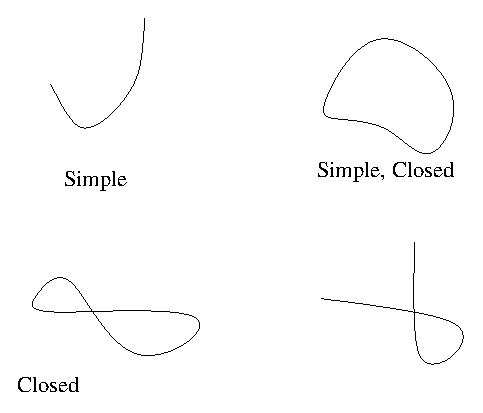
\includegraphics{curves.eps}}
\end{center}
\caption{Examples of paths}
\end{figure} 

\section{Complex Integration}

A function $f \colon [a,b] \mapsto \C$ is said to be Riemann integrable if both
its real and imaginary parts are Riemann integrable.  The integral is defined
to be
\[
\int_a^b f(t) \ud t = \int_a^b \Re(f(t)) \ud t + \imath \int_a^b \Im(f(t)) \ud t.
\]

\begin{lemma}
Let $f \colon [a,b] \mapsto \C$ be continuous.  Then
\[
\abs{\int_a^b f(t) \ud t} \le \int_a^b \abs{f(t)} \ud t.
\]
\end{lemma}

\begin{proof}
For suitable $\theta \in \R$,
\begin{align*}
\abs{\int_a^b f(t) \ud t} &= e^{\imath \theta} \int_a^b f(t) \ud t
= \int_a^b e^{\imath \theta} f(t) \ud t \\
&= \Re \int_a^b e^{\imath \theta} f(t) \ud t = \int_a^b \Re(e^{\imath \theta}
f(t)) \ud t \\
&\le \int_a^b \abs{f(t)} \ud t \quad \text{using the real result.}
\end{align*}
\end{proof}

\section{Domains}

\begin{definition}
A domain\index{domain} is a connected open subset of $\C$.
\end{definition}

\begin{examples}
Some examples of domains are
\begin{enumerate}
\item $\C$,
\item $\Delta = \{ z : \abs{z} < 1 \}$,
\item $\C \setminus \{ 0 \}$,
\item $\{ z : a < \abs{z} < b \}$.
\end{enumerate}
\end{examples}

\begin{definition}
Given $x, y \in \C$, let $[x \rightarrow y]$ be the path $\phi \colon [0,1] \mapsto
\C$, $\phi(t) = (1-t) x + t y$.
\end{definition}

\begin{definition}
A domain $D$ is convex\index{domain!convex} if
$x, y \in D \Rightarrow [x \rightarrow y]^* \subset D$.
\end{definition}

\begin{definition}
A domain $D$ is star-shaped\index{domain!star-shaped}
if $\exists\ z_0 \in D$ such that
$[z_0 \rightarrow z]^* \subset D\ \forall\ z \in D$.
\end{definition}

\begin{figure}[h]
\begin{center}
\scalebox{0.75}{
\includegraphics{domains.eps}}
\end{center}
\caption{Examples of domains}
\end{figure}

A star-shaped domain is sometimes called a star-domain.  Note that every
(non-empty) convex domain is star-shaped.

\section{Path Integrals}

\begin{definition}
Let $D$ be a domain, $f \colon D \mapsto \C$ be continuous and $\phi \colon [a,b]
\mapsto D$ be a smooth path.  Then the integral of $f$ along $\phi$ is defined
as
\[
\int_\phi f(z) \ud z = \int_a^b f(\phi(t)) \phi'(t) \ud t.
\]

If $\phi$ is piecewise smooth, then pick $a = x_0 < \dots < x_n = b$ such
that $\phi \bigr|_{[x_{i-1},x_i]}$ is smooth and then
\[
\int_\phi f(z) \ud z = \sum_{i=1}^n \int_{x_{i-1}}^{x_i} f(\phi(t)) \phi'(t) \ud t.
\]
\end{definition}

\begin{lemma}
Equivalent paths give the same integral.
\end{lemma}

\begin{proof}
Let $D$ be a domain and $\phi \colon [a,b] \mapsto D$ and $\psi \colon [c,d] \mapsto
D$ be equivalent smooth paths.  Let $f \colon D \mapsto \C$ be continuous and
$\gamma \colon [a,b] \mapsto [c,d]$ give the equivalence.  Then
\begin{align*}
\int_\psi f(z) \ud z &= \int_c^d f(\psi(s)) \psi'(s) \ud s =
\int_a^b f(\psi(\gamma(t))) \psi'(\gamma(t)) \gamma'(t) \ud t \\
&= \int_a^b f(\phi(t)) \phi'(t) \ud t = \int_\phi f(z) \ud z.
\end{align*}

If $\phi$ and $\psi$ are piecewise smooth write $\phi = \phi_1 \vee \dots
\vee \phi_n$ and $\psi = \psi_1 \vee \dots \vee \psi_n$, with $\phi_i$ and
$\psi_i$ smooth, $\phi_i$ equivalent to $\psi_i$.  Then

\[
\int_\phi f(z) \ud z = \sum_{i=1}^n \int_{\phi_i} f(z) \ud z
= \sum_{i=1}^n \int_{\psi_i} f(z) \ud z = \int_\psi f(z) \ud z.
\]
\end{proof}

\begin{example}
Let $D$ be $\C \setminus \{ 0 \}$ and $f(z) = z^n$ for some $n \in \Z$, 
$\phi \colon [0,2 \pi ] \mapsto D$ be $t \mapsto e^{\imath t}$.  Then
\[
\int_\phi f(z) \ud z = 
\begin{cases}
2 \pi \imath & \text{if } n = -1 \\
0 & \text{otherwise.}
\end{cases}
\]
\end{example}

\begin{proof}
\begin{align*}
\int_\phi f(z) \ud z &= \int_0^{2 \pi} e^{n \imath t} \imath e^{\imath t} \ud t 
= \imath \int_0^{2 \pi} e^{(n+1) \imath t} \ud t \\
&= \begin{cases}
\left[ \frac{e^{(n+1) \imath t}}{n+1} \right]_0^{2 \pi} = 0 & \text{if }
n \neq -1 \\
2 \pi \imath & \text{if } n = -1.
\end{cases}
\end{align*}
\end{proof}

\begin{definition}
Let $D$ be a domain and $\phi \colon [a,b] \mapsto D$ be a smooth path.  Then
the length of $\phi$, $L(\phi)$ is defined as
\[
L(\phi) = \int_a^b \abs{\phi'(t)} \ud t.
\]
\end{definition}

\begin{lemma}
Let $D$ be a domain, $f \colon D \mapsto \C$ be continuous and $\phi \colon [a,b]
\mapsto D$ be a smooth path.  Then
\[
\abs{\int_\phi f(z) \ud z} \le \sup_{z \in \phi^*} \abs{f(z)} L(\phi).
\]
\end{lemma}

\begin{proof}
\begin{align*}
\abs{\int_\phi f(z) \ud z} &= \abs{\int_a^b f(\phi(t)) \phi'(t) \ud t} \\
&\le \int_a^b \abs{f(\phi(t))} \abs{\phi'(t)} \ud t \\
&\le \sup_{z \in \phi^*} \abs{f(z)} L(\phi) \quad \text{by real result}.
\end{align*}
\end{proof}

\begin{remark}
The above generalises easily to piecewise smooth paths.
\end{remark}

Henceforth, all paths are piecewise smooth unless otherwise stated.

\begin{proposition}[Fundamental Theorem of Calculus]%
\index{Fundamental Theorem of Calculus}
Let $D$ be a domain and let $f \colon D \mapsto \C$ be continuous.  Suppose
$f$ has an antiderivative $F$ (i.e. a function $F(z)$ such that
$F'(z) = f(z)\ \forall\ z \in D$).  Let $\phi \colon [a,b] \mapsto D$ be a
path.  Then
\[
\int_{\phi} f(z) \ud z = F(\phi(b)) - F(\phi(a)).
\]
\end{proposition}

\begin{proof}
If $\phi$ is smooth, then
\[
\int_\phi f(z) \ud z = \int_a^b f(\phi(t))\phi'(t) \ud t = \int_a^b
(F \circ \phi)'(t) \ud t = F \circ \phi (b) - F \circ \phi(a).
\]
In general if $a = x_0 < x_1 < \dots < x_n = b$ and $\phi \bigr|_{[x_{i-1},
x_i]}$ is smooth, then the above argument gives that
\[
\int_\phi f(z) \ud z = \sum_{i=1}^n (F(\phi(x_i)) - F(\phi(x_{i-1}))) =
F(\phi(b)) - F(\phi(a)).
\]
\end{proof}

\begin{corollary}
If $D$ is a domain, $f \colon D \mapsto \C$ is continuous with antiderivative
$F$ and $\phi$ is a closed path, then
\[
\int_\phi f(z) \ud z = 0.
\]
\end{corollary}

\begin{proof}
Immediate.
\end{proof}

\begin{lemma}
Let $D$ be a star-domain and $f \colon D \mapsto \C$ be continuous.  Then the
following are equivalent.
\begin{enumerate}
\item $f$ has an antiderivative $F$ on $D$.
\item $\int_\phi f(z) \ud z = 0$ for all closed paths $\phi$ in $D$.
\item $\int_{\partial T} f(z) \ud z = 0$ for the boundary $\partial T$ of
any triangle $T$ such that $T \subset D$ \footnote{Including the boundary
and interior.}.
\end{enumerate}
\end{lemma}

\begin{proof}
It is enough to do $3 \Rightarrow 1$.  Take $z_0 \in D$ such that
$[z_0 \rightarrow z]^* \subset D\ \forall\ z \in D$ and define
\[
F(z) = \int_{[z_0 \rightarrow z]^*} f(w) \ud w.
\]

Then take $T$ to be the triangle with vertices $z_0$, $z$ and $z+h$.  Since
$D$ is open, $[z \rightarrow z+h]^* \subset D$ for $\abs{h}$ sufficiently
small which gives that $T \subset D$.  Now 
\[
F(z+h)-F(z) = \int_{[z \rightarrow z+h]^*} f(w) \ud w, \text{ so that}
\]
\begin{align*}
\abs{F(z+h)-F(z) - h f(z)} 
&= \abs{ \int_{[z \rightarrow z+h]^*} (f(w)-f(z)) \ud w} \\
&\le \sup_{w \in [z \rightarrow z+h]} \abs{f(w)-f(z)} \abs{h}. \\
\intertext{Choose $\delta > 0$ such that $\abs{h} < \delta \Rightarrow
\abs{f(z+h)-f(z)} < \epsilon$. Then}
\abs{F(z+h)-F(z) - h f(z)} &\le \epsilon \abs{h}.
\end{align*}
\end{proof}

\chapter{Cauchy's theorem and its consequences}

\section{Cauchy's theorem}

\begin{definition}
Let $D$ be a domain and $f \colon D \mapsto \C$ be continuous.  $f$ is
analytic\index{analytic} (or holomorphic\index{holomorphic})%
\footnote{Outside Cambridge, an analytic
function is one which has a power series expansion and a holomorphic
function is $\C$ differentiable on a domain.}
if $f$ is differentiable at $z\ \forall z \in D$.
\end{definition}

\begin{theorem}[Cauchy's theorem for triangles]%
\index{Cauchy's Theorem!for triangles}
Let $D$ be a domain and $T$ be a triangle lying entirely in $D$.  If
$f \colon D \mapsto \C$ is analytic, then
\[
\int_{\partial T} f(z) \ud z = 0.
\]
\end{theorem}

\begin{proof}
Let $\eta = \abs{\int_{\partial T} f(z) \ud z}$ and let $l = L(\partial T)$.
Now let $T_0 = T$.  We can split $T$ into 4 equally sized triangles
$T^1, T^2, T^3, T^4$ as shown, with all boundaries oriented in the same
direction as that of $T$.

\begin{figure}[h]
\begin{center}
\scalebox{0.75}{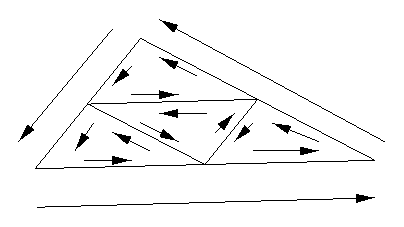
\includegraphics{tri.eps}}
\end{center}
\caption{Splitting up the triangle}
\end{figure}

Since the contributions from internal edges cancel, 
\[
\int_{\partial T} f(z) \ud z = \sum_{i=1}^4 \int_{\partial T^i} f(z) \ud z,
\]
and $\exists\ i \le 4$ such that
\[
\abs{\int_{\partial T^i} f(z) \ud z} \ge \frac{\eta}{4}.
\]
Put $T_1 = T^i$ for this $i$ and repeat the process.  We produce a sequence
$T_0$, $T_1$, $T_2$, $\dots$ such that
\[
\abs{\int_{\partial T_n} f(z) \ud z} \ge \frac{\eta}{4^n} \text{ and }
\]
\[
L(\partial T_n) = \frac{l}{2^n}.
\]
Since the $T_n$ are closed, we can find $z_0 \in \bigcap_{i=1}^\infty T_n$.
As $f$ is differentiable at $z_0$, $\forall\ \epsilon > 0, \exists\ \delta
> 0$ such that
\[
\abs{w-z_0} < \delta \Rightarrow \abs{f(w) - f(z_0)
- (w-z_0)f'(z_0)} < \epsilon \abs{w-z_0}.
\]
Pick $n$ such that $T_n \subset B_\delta (z_0)$.  Then
\begin{align*}
\abs{\int_{\partial T_n} f(z) \ud z}
&= \abs{\int_{\partial T_n} (f(z) - f(z_0) - (z-z_0) f'(z_0)) \ud z} \\
&\le L(\partial T_n) \epsilon \sup_{z \in \partial T_n} \abs{z-z_0} \\
&\le \epsilon L(\partial T_n)^2.
\end{align*}
But $\abs{\int_{\partial T_n} f(w) \ud w} \ge 4^{-n} \eta l^2$.  This gives
that $\eta < \epsilon$.  But $\epsilon > 0$ is arbitrary, so $\eta = 0$.
\end{proof}

\begin{corollary}[Cauchy's Theorem for a star-domain]%
\index{Cauchy's Theorem!for a star-domain}
Let $D$ be a star-domain and $f \colon D \mapsto \C$ be analytic.  Then
\[
\int_\phi f(z) \ud z = 0 \text{ for all closed paths $\phi$ in $D$.}
\]
\end{corollary}

\begin{proof}
Result true for triangles.  Thus $f$ has an anti-derivative and thus
\[
\int_\phi f(z) \ud z = 0.
\]
\end{proof}

\section{Homotopy}

\begin{definition}
Let $\phi \colon [0,1] \mapsto D$ and $\psi \colon [0,1] \mapsto D$ be piecewise smooth
closed paths in a domain $D$.  A homotopy\index{homotopy} from $\phi$ to
$\psi$ is a function $\gamma \colon [0,1]^2 \mapsto D$ such that
\begin{enumerate}
\item $\gamma$ is continuous,
\item $\gamma(0,t) = \phi(t)\ \forall\ t \in [0,1]$,
\item $\gamma(1,t) = \psi(t)\ \forall\ t \in [0,1]$,
\item $\forall\ s \in [0,1]$, the path $\gamma_s(t)$ defined by $\gamma_s(t)
= \gamma(s,t)$ is closed and piecewise smooth.
\end{enumerate}
\end{definition}

\begin{figure}[h]
\begin{center}
\scalebox{0.75}{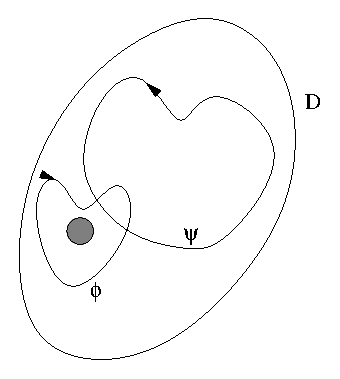
\includegraphics{nonhom.eps}}
\end{center}
\caption{Two non-homotopic paths.}
\end{figure}

\begin{definition}
$\psi$ is said to be an elementary deformation%
\index{elementary deformation} of $\phi$ if
$\exists\ 0 = x_0 < x_1 < \dots < x_n = 1$ and convex open subsets
$C_1, \dots, C_n \subset D$ such that $x_{i-1} \le t \le x_i
\Rightarrow \phi(t) \in C_i, \psi(t) \in C_i$.
\end{definition}

\begin{figure}[h]
\begin{center}
\scalebox{0.50}{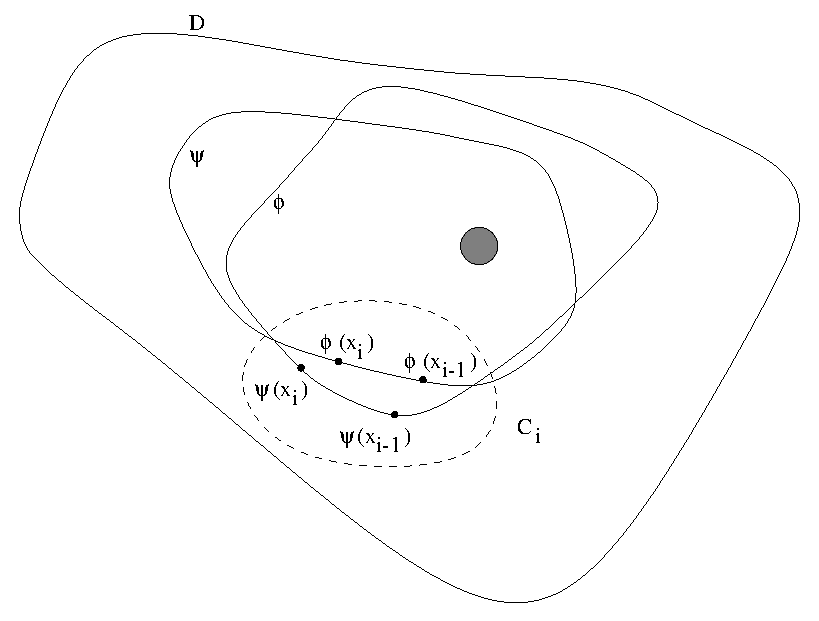
\includegraphics{eldef.eps}}
\end{center}
\caption{Elementary deformation}
\end{figure}

\begin{lemma}
  Let $D$ be a domain, $f \colon D \mapsto \C$ be analytic, $\phi
  \colon [0,1] \mapsto D$ be a closed path and $\psi$ be an elementary
  deformation of $\phi$.  Then
\[
\int_\phi f(z) \ud z = \int_\psi f(z) \ud z.
\]
\end{lemma}

\begin{proof}
Let $\phi_i$ and $\psi_i$ be the restrictions to $[x_{i-1},x_i]$ of $\phi$ and
$\psi$ respectively.  Let $\gamma_i = [\phi(x_i) \rightarrow \psi(x_i)]$.
By Cauchy's theorem for a star-domain,
\[
\int_{\phi_i} f(z) \ud z + \int_{\gamma_i} f(z) \ud z
- \int_{\psi_i} f(z) \ud z - \int_{\gamma_{i-1}} f(z) \ud z = 0.
\]
Now summing from $i = 1 \dots n$ gives that
\[
\int_\phi f(z) \ud z = \int_\psi f(z) \ud z.
\]
\end{proof}

\begin{proposition}
Let $D$ be a domain and let $\phi \colon [0,1] \mapsto D$ and
$\psi \colon [0,1] \mapsto D$ be homotopic.  Then
$\exists\ \phi = \phi_0, \phi_1, \dots, \phi_n = \psi$ such that
$\phi_i$ is an elementary deformation of $\phi_{i-1}$.
\end{proposition}

\begin{proof}
Let $\gamma \colon [0,1]^2 \mapsto D$ be a homotopy from $\phi$ to $\psi$.
$[0,1]^2$ is compact, so $\gamma([0,1]^2)$ is a compact subset of $D$.
Now $\C \setminus D$ is closed and disjoint from $\gamma([0,1]^2)$ so
$\exists\ \epsilon > 0$ such that $\forall\ z \in \gamma([0,1]^2)
\text{ and } w \notin D, \abs{z-w} \ge \epsilon$.  Thus $\forall
(s,t) \in [0,1]^2$, $B_\epsilon(\gamma(s,t)) \subset D$.
Also, $\gamma$ is uniformly continuous on $[0,1]^2$, so $\exists\ \delta
> 0$ such that
\[
\left(
(s-s')^2 + (t-t')^2
\right)^{1/2} < \delta
\Rightarrow
\abs{\gamma(s,t) - \gamma(s',t')} < \epsilon.
\]

Now pick $n \in \N$ such that $\frac{2}{n} < \delta$ and let $\phi_i =
\gamma_{\frac{i}{n}}, i = 0, \dots, n$.  Let $x_j = \frac{j}{n}$ and
$C_{ij} = B_\epsilon (\gamma(x_i,x_j))$.

But if $\frac{i-1}{n} \le s \le \frac{i}{n}$ and $\frac{j-1}{n} \le t \le
\frac{j}{n}$ then 
\[
\left(
(s-s')^2 + (t-t')^2
\right)^{1/2} < \frac{2}{n} < \delta
\Rightarrow
\abs{\gamma(s,t) - \gamma(i/n,j/n)} < \epsilon
\Rightarrow \gamma(s,t) \in C_{ij}.
\]

Thus $\phi_i$ is an elementary deformation of $\phi_{i-1}$.
\end{proof}

\begin{corollary}
Let $D$ be a domain, $f \colon D \mapsto \C$ be analytic and $\phi$, $\psi$ be
homotopic closed paths in $D$.  Then
\[
\int_\phi f(z) \ud z = \int_\psi f(z) \ud z.
\]
\end{corollary}

\begin{proof}
Immediate from above.
\end{proof}

\begin{definition}
Let $D$ be a domain.  A closed path $\phi$ is contractible%
\index{path!contractible} if it is homotopic to a constant path.
\end{definition}

\begin{definition}
A domain $D$ is simply connected\index{domain!simply connected} if every
closed path is contractible. 
\end{definition}

\begin{corollary}[Cauchy's theorem for a simply connected domain]%
\index{Cauchy's Theorem!for a simply connected domain}\hfill\\
Let $D$ be a domain and $f \colon D \mapsto \C$ be analytic.  If the closed
path $\phi$ is contractible, then
\[
\int_\phi f(z) \ud z = 0.
\]

If $D$ is simply connected then
\[
\int_\phi f(z) \ud z = 0 \text{ for all closed paths $\phi$.}
\]
\end{corollary}

\begin{proof}
Immediate.
\end{proof}

\begin{notation}
\begin{align*}
B_r(z_0) \equiv B(z_0,r) & \equiv \{ z \in \C : \abs{z-z_0} < r \} \\
\text{thus } \overline{B_r(z_0)} \equiv \overline{B(z_0,r)} & \equiv
\{ z \in \C : \abs{z-z_0} \le r \}.
\end{align*}

$C(z_0,r) \equiv C_r(z_0)$ is the path $t \mapsto z_0 + r e^{2 \pi \imath t}$
for $t \in [0,1]$.
\end{notation}

\section{Consequences of Cauchy's Theorem}

\begin{theorem}[Cauchy's Integral Formula]%
  \index{Cauchy's Integral Formula} Let $D$ be a domain and let $f
  \colon D \mapsto \C$ be analytic.  Let $z_0$, $r$ be such that
  $\overline{B_r(z_0)} \subset D$.  Then $\forall\ z \in B_r(z_0)$,
\[
f(z) = \frac{1}{2 \pi \imath} \int_{C_r(z_0)} \frac{f(w)}{w-z} \ud w.
\]
\end{theorem}

\begin{figure}[h]
\begin{center}
\scalebox{0.75}{
\includegraphics{balls.eps}}
\end{center}
\end{figure}

\begin{proof}
Take $\epsilon > 0$.  Let $\delta > 0$ be such that $\overline{B_\delta(z)}
\subset B_r(z_0)$ and $\abs{w-z} = \delta \Rightarrow \abs{f(w) - f(z)} \le
\epsilon$.  Then
\begin{align*}
\abs{f(z) - \frac{1}{2 \pi \imath} \int_{C_r(z_0)} \frac{f(w)}{w-z} \ud w}
&=
\abs{f(z) - \frac{1}{2 \pi \imath} \int_{C_\delta(z)} \frac{f(w)}{w-z} \ud w} \\
\intertext{ since $\gamma(s,t) = (1-s) (z_0 + r e^{2 \pi \imath t}) +
 s (z +  \delta e^{2 \pi \imath t})$ is a homotopy from $C_r (z_0)$ to
$C_\delta(z)$ in $D \setminus \{ z \}$ in which $\frac{f(w)}{w-z}$ is
analytic.  Thus}
&= \abs{\frac{1}{2 \pi \imath}
\int_{C_\delta(z)} \frac{f(z) - f(w)}{w-z} \ud w} \\
& \le \frac{1}{2 \pi} \frac{ 2 \pi \delta \epsilon}{\delta} = \epsilon.
\end{align*}
But $\epsilon > 0$ is arbitrary, so result follows.
\end{proof}

\begin{remark}
Note that the proof of Cauchy's integral formula given does not need the
full strength of homotopy invariance, since $C_\delta(z)$ is clearly an
elementary deformation of $C_r(z_0)$
\end{remark}

\begin{theorem}[Liouville's Theorem]%
\index{Liouville's Theorem}
Every bounded entire function is constant.
\end{theorem}

\begin{proof}
  Let $f \colon \C \mapsto \C$ be analytic and $\abs{f(z)} \le M\ 
  \forall\ z \in \C$.  Take $z_1, z_2 \in \C$ and let $R \ge 2 \max \{
  \abs{z_1}, \abs{z_2} \}$.  Then

\begin{align*}
\abs{f(z_1) - f(z_2)} &=
\abs{\frac{1}{2 \pi \imath} \int_{C_R(0)} \left(
\frac{f(w)}{w-z_1} - \frac{f(w)}{w-z_2}
\right) \ud w} \\
&= \abs{\frac{1}{2 \pi \imath} \int_{C_R(0)} \frac{f(w)(z_1 - z_2)}{(w-z_1)
(w-z_2)} \ud w} \\
&\le \frac{1}{2 \pi} \frac{2 \pi R M \abs{z_1 - z_2}}{\left(\frac{R}{2}
\right)^2} \\
&= \frac{4 M \abs{z_1 - z_2}}{R}.
\end{align*}

But $R$ can be arbitrarily large, so result follows.
\end{proof}

\begin{theorem}[The Fundamental Theorem of Algebra]
  \index{Fundamental Theorem of Algebra} Every non-constant polynomial
  has at least one root in $\C$.
\end{theorem}

\begin{proof}
  Let $p$ be a non-constant polynomial and suppose that $p$ has no
  roots.  Then the function $\frac{1}{p(z)}$ is analytic on $\C$.
  Suppose that
\[
p(z) = a_n z^n + \dots + a_0, \text{ with } a_n \neq 0.
\]

Then if
\[
\abs{z} \ge
\max \left\{ 1 , 2 \frac{ \abs{a_{n-1}} + \dots + \abs{a_0} }{ \abs{a_n} }
\right\}, \]
\begin{align*}
\abs{p(z)} &\ge \abs{a_n} \abs{z}^n - \left(\abs{a_{n-1}} + \dots + \abs{a_0}
\right) \abs{z}^{n-1} \\
&\ge \frac{1}{2} \abs{a_n} \abs{z}^n \ge \frac{1}{2} \abs{a_n}.
\end{align*}
So $\exists\ M$ such that $\abs{z} \ge M \Rightarrow \abs{\frac{1}{p(z)}}
\le \frac{2}{a_n}$.  Now $\frac{1}{p(z)}$ is continuous and
$\overline{B_M(0)}$ is compact, so $\frac{1}{p}$ is bounded in
$\overline{B_M(0)}$.  Hence $\frac{1}{p}$ bounded on all of $\C$ and thus
constant.  This is a contradiction.
\end{proof}

\begin{proposition}
Let $g$ be a continuous function from $\{ z \in \C : \abs{z - z_0} = r \}$ to
$\C$.  Then
\[
f(z) = \int_{C_r(z_0)} \frac{g(w)}{\left( w - z \right)^n} \ud w
\]
is analytic on $B_r(z_0)$ and
\[
f'(z) = n \int_{C_r(z_0)} \frac{g(w)}{\left( w - z \right)^{n+1}} \ud w
\]
\end{proposition}

\begin{proof}
Let $2 \epsilon = r - \abs{z - z_0}$ such that $\abs{w - z_0} = r
\Rightarrow \abs{w - z} \ge 2 \epsilon$.  Now

\begin{align*}
&\abs{ \frac{1}{\left( w - z -h \right)^n} - \frac{1}{\left( w - z \right)^n}}
= \\
&\quad \abs{ \left( \frac{1}{w-z-h} - \frac{1}{w-z} \right)
\sum_{k=0}^{n-1} \frac{1}{\left(w-z-h\right)^k \left(w-z\right)^{n-1-k}} } \\
& \quad =
\abs{ \frac{h}{\left(w-z-h\right) \left(w-z \right)}
\sum_{k=0}^{n-1} \frac{1}{\left(w-z-h\right)^k \left(w-z\right)^{n-1-k}} } \\
&\quad \le \frac{h n}{\epsilon^{n+1}} \\
&\quad \rightarrow 0 \text{ as } \abs{h} \rightarrow 0 \text{ independently of } w.
\end{align*}

When $\abs{h} \le \epsilon$,
\begin{align*}
& \abs{f(z+h)  - f(z) - h n \int_{C_r(z_0)} \frac{g(w)}{\left( w-z \right)^{n+1}}
\ud w}
= \\ 
&\quad \abs{
\int_{C_r(z_0)} h g(w) \left(
\frac{1}{\left(w-z-h\right) \left(w-z \right)}
\sum_{k=0}^{n-1} \frac{1}{\left(w-z-h\right)^k \left(w-z\right)^{n-1-k}}
\right) \ud w}
\end{align*}

Using the same estimate as above, the bit in brackets converges to $0$
as $h \rightarrow 0$.  Since $g(w)$ is bounded on $C_r(z_0)^*$ for
$\abs{h}$ sufficiently small the whole integral is at most $\epsilon \abs{h}$.
\end{proof}

\begin{corollary}
Let $D$ be a domain and $f \colon D \mapsto \C$ be analytic.  Then $f$ is
infinitely differentiable inside $B_r(z_0)$, $\overline{B_r(z_0)} \subset D$
and $\forall\ z \in B_r(z_0),$
\[
f^{(n)}(z) = \frac{n!}{2 \pi \imath} \int_{C_r(z_0)} \frac{f(w)}{\left(
w-z \right)^{n+1}} \ud w.
\]
\end{corollary}

\begin{proof}
The case $n=0$ is Cauchy's integral formula.  If we have it for $n$, then
the proposition gives it for $n+1$.
\end{proof}

\begin{theorem}[Morera's Theorem]
\index{Morera's Theorem}
Let $D$ be a star-shaped domain and \\ $f \colon D \mapsto \C$ be continuous.
If
\[
\int_{\partial T} f(z) \ud z = 0
\]
for all triangles $T \subset D$ then $f$ is analytic.
\end{theorem}

\begin{proof}
The condition implies that $f$ has an antiderivative $F$, which is analytic.
$F$ is therefore infinitely differentiable, so $f$ is analytic.
\end{proof}

\begin{remark}
Now let $D$ be an arbitrary domain and let $z \in D$.  Since $\exists\ \epsilon
> 0$ such that $B_\epsilon(z) \subset D$ and $B_\epsilon(z)$ is star-shaped,
one can easily extend Morera's Theorem to any domain.
\end{remark}

\chapter{Power Series}

\section{Analyticity and Holomorphy}

\begin{lemma}
Consider a power series $\sum_{n=0}^\infty a_n (z-z_0)^n$.  If this sum
converges for some $z$ with $\abs{z-z_0} = \rho$, then it converges for all
$w$ with $\abs{w-z_0} < \rho$ and for any $r < \rho$, the convergence is
uniform in $\overline{B_r(z_0)}$.
\end{lemma}

\begin{proof}
Since $\sum_{n=0}^\infty a_n (z-z_0)^n$ converges, then
$\exists\ M$ such that $\abs{a_n}\abs{z-z_0}^n = \abs{a_n} \rho^n \le M\
\forall\ n$.  If $\abs{w-z_0} < \rho$, then
\begin{align*}
\abs{\sum_{n=N}^\infty a_n (w-z_0)^n} &\le
M \sum_{n=N}^\infty \abs{\frac{w-z_0}{\rho}}^n \\
&\le \sum_{n=N}^\infty \left(\frac{r}{\rho}\right)^n \\
&= M \left( \frac{r}{\rho} \right)^n \frac{1}{1-\frac{r}{\rho}} \\
&\rightarrow 0 \text{ independently of $w$.}
\end{align*}
\end{proof}

\begin{definition}
The radius of convergence\index{radius of convergence} of a power series
$\sum_{n=0}^\infty a_n (z-z_0)^n$ is
\[
R = \sup \{ r : \exists\ z \text{ such that } \abs{z-z_0} < r \text{ and }
\sum_{n=0}^\infty a_n (z-z_0)^n \text{ converges.}\}.
\]
\end{definition}

\begin{lemma}
Let $D$ be a domain, $\phi \colon [a,b] \mapsto D$ be a path and $f_n \colon D \mapsto
\C$ be continuous.  Suppose $f_n \rightarrow f$ uniformly on $\phi^*$.  Then
\[
\int_\phi f_n(z) \ud z \rightarrow \int_\phi f(z) \ud z.
\]
\end{lemma}

\begin{proof}
Let $\epsilon > 0$.  Then $\exists\ N$ such that $\forall\ n \ge N\
\forall\ z \in \phi^*$, $\abs{f_n(z)-f(z)} \le \frac{\epsilon}{L(\phi)}$.
Then
\begin{align*}
\abs{\int_\phi f_n(z) \ud z - \int_\phi f(z) \ud z} &=
\abs{\int_\phi f_n - f \ud z} \\
&\le \epsilon.
\end{align*}

But $\epsilon > 0$ is arbitrary, so result follows. 
\end{proof}

\begin{lemma}
Let $f(z) = \sum_{n=0}^\infty a_n (z-z_0)^n$ and
$g(z) = \sum_{n=0}^\infty b_n (z-z_0)^n$.  Suppose there exists a sequence
$(z_k)_{k=1}^\infty \rightarrow z_0$, $z_k \neq z_0$ and $f(z_k) = g(z_k)$.
Then $a_n = b_n$ for all $n$.
\end{lemma}

\begin{proof}
Suppose otherwise.  Then let $N$ be minimal such that $a_N \neq b_N$.  Now
let $c_n = a_n - b_n$.  Then
\begin{align*}
f(z) - g(z) &= \sum_{n=N}^\infty c_n (z-z_0)^n \\
&= (z-z_0)^n \left( c_N + \left( z-z_0 \right) 
\sum_{n=N+1}^\infty c_n (z-z_0)^{n-N-1} \right).
\end{align*}

For $\abs{z_0 - z_k}$ sufficiently small, then 
\[
\abs{z_k - z_0} \abs{\sum_{n=N+1}^\infty c_n (z-z_0)^{n-N-1}} < \frac{1}{2}
\abs{c_N}
\]
and thus $f(z_k) - g(z_k) \neq 0$.
\end{proof}

\begin{lemma}
Let $f(z) = \sum_{n=0}^\infty a_n (z-z_0)^n$ with radius of convergence $R$.
Then $f$ is analytic in $B_R(z_0)$ and
$f'(z) = \sum_{n=1}^\infty n a_n (z-z_0)^{n-1}$. 
\end{lemma}

\begin{proof}
Let $z \in B_R(z_0)$.  Pick $r$ such that $\abs{z-z_0} < r < R$.  Let
\[
f_N(z) = \sum_{n=0}^N a_n (z-z_0)^n.
\]
Then $f_N \rightarrow f$ uniformly
on $\overline{B_r(z_0)}$.  Since $\abs{w - z_0} = r \Rightarrow
\abs{w-z} \ge r - \abs{z-z_0}$, we have \[
\frac{f_N(w)}{w-z} \rightarrow \frac{f(w)}{w-z} \quad \text{and }
\frac{f_N(w)}{(w-z)^2} \rightarrow \frac{f(w)}{(w-z)^2} \text{ uniformly for }
\abs{w-z_0} = r.
\]
But \[
f_N(z) = \frac{1}{2 \pi \imath} \int_{C_r(z_0)} \frac{f_N(w)}{w-z} \ud w
\rightarrow \frac{1}{2 \pi \imath} \int_{C_r(z_0)} \frac{f(w)}{w-z} \ud w.
\]
Therefore \[
f(z) = \frac{1}{2 \pi \imath} \int_{C_r(z_0)} \frac{f(w)}{w-z} \ud w.
\]
Hence $f$ is differentiable at $z$ and \[
f'(z) = \frac{1}{2 \pi \imath} \int_{C_r(z_0)} \frac{f(w)}{(w-z)^2} \ud w.
\]
Also, \[
f_N'(z) = \frac{1}{2 \pi \imath} \int_{C_r(z_0)} \frac{f_N(w)}{(w-z)^2} \ud w
\rightarrow \frac{1}{2 \pi \imath} \int_{C_r(z_0)} \frac{f(w)}{(w-z)^2} \ud w
= f'(z).
\]
Hence $f'(z) = \sum_{n=1}^\infty n a_n (z-z_0)^n$ as claimed.
\end{proof}

\begin{theorem}[Taylor's Theorem]%
\index{Taylor's Theorem}
Let $D$ be a domain and then $f \colon D \mapsto \C$ be analytic.  Let $z_0 \in D$
and let $R$ be such that $B_R(z_0) \subset D$.  Then there exist unique
coefficients $(a_n)_{n=0}^\infty$ such that
\[
f(z) = \sum_{n=0}^\infty a_n (z-z_0)^n\ \forall\ z \in B_R(z_0).
\]
\end{theorem}

\begin{proof}
Let $z \in B_R(z_0)$ and let $r$ be such that $\abs{z-z_0} < r < R$.  Then
by Cauchy's integral formula,
\begin{align*}
f(z) &= \frac{1}{2 \pi \imath} \int_{C_r(z_0)} \frac{f(w)}{w-z} \ud w \\
&= \frac{1}{2 \pi \imath} \int_{C_r(z_0)} \frac{f(w)}{(w-z_0) - (z-z_0)} \ud w \\
&= \frac{1}{2 \pi \imath} \int_{C_r(z_0)} \frac{f(w)}{w-z_0}
\frac{1}{1- \frac{z-z_0}{w-z_0}} \ud w \\
&= \frac{1}{2 \pi \imath} \int_{C_r(z_0)} \frac{f(w)}{w-z_0}
\sum_{n=0}^\infty \left( \frac{z-z_0}{w-z_0} \right)^n \ud w.
\end{align*}
As $\abs{\frac{z-z_0}{w-z_0}} < 1$, the convergence is uniform, so can
exchange the sum and integral to get
\[
f(z) = \sum_{n=0}^\infty \frac{\left( z - z_0 \right)^n}{2 \pi \imath}
\int_{C_r(z_0)} \frac{f(w)}{\left( w - z_0 \right)^{n+1}} \ud w.
\]
To get uniqueness use above lemma.
\end{proof}

\begin{theorem}[Identity Theorem]%
\index{Identity Theorem}
Let $D$ be a domain and $f,g \colon D \mapsto \C$ be analytic.  Suppose 
$z_k \rightarrow z_0 (\in D)$, $z_k \neq z_0$ and $f(z_k) = g(z_k)$
for all $k$.  Then $f(z) = g(z)\ \forall\ z \in D$.  In particular,
setting $g \equiv 0$ gives that the zeros of a non-constant analytic function
are isolated.
\end{theorem}

\begin{proof}
Define $U = \{ z \in D : f^{(n)} (z) = g^{(n)} (z)\ \forall n\}$.  Now 
$U \ne \emptyset$ since $z_0 \in U$ as the earlier result on uniqueness of
power series implies that the Taylor expansions of $f$ and $g$ at $z_0$ are
the same.

Now $U$ is closed, since
\[
U = \bigcap_{n=0}^\infty \left ( f^{(n)} - g^{(n)} \right)^{-1} \left( \{ 0 \}
\right).
\]
If $z \in U$, then the Taylor expansions of $f$ and $g$ agree at $z$, so
$f \equiv g$ in some $B_\delta(z)$ and then for $y \in B_\delta(z)$, $f$ and
$g$ must have the same $n^{th}$ derivatives at $y$.  Thus $U$ is open and
since $D$ is connected, $U = D$. 
\end{proof}

\begin{proposition}
Let $D$ be a domain, $z_0 \in D$ and $f \colon D \mapsto \C$ be analytic such that
$f \not \equiv 0$.  Then there exist a unique $k \ge 0$ and a unique analytic
function $g$ such that $g(z_0) \neq 0$ and $f(z) = (z - z_0)^k g(z)$.
\end{proposition}

\begin{proof}
Let the Taylor expansion of $f$ at $z_0$ be $\sum_{n=0}^\infty a_n (z-z_0)^n$.
Now choose $N$ minimal such that $a_N \neq 0$.  (This is do-able since $f \not
\equiv 0$.)  Thus we can write 
\[
f(z) = (z-z_0)^N \sum_{n=0}^\infty a_{n+N} (z-z_0)^n
\]
in some $B_\delta(z_0)$.  Set
\[
g(z) = \begin{cases}
\sum_{n=0}^\infty a_{n+N} (z-z_0)^n & \text{if } \abs{z-z_0} < \delta \\
(z - z_0)^{-N} f(z) & \text{if } z \neq z_0.
\end{cases}
\]
These two cases agree when $0 < \abs{z-z_0} < \delta$ and 
$f(z) = (z-z_0)^N g(z)$, $g(z_0) = a_N \neq 0$.  Now if 
$f(z) = (z-z_0)^{k_1} g_1(z) = (z-z_0)^{k_2} g_2(z)\ \forall\ z \in D$,
take $k_1 \le k_2$ without loss of generality.  Then for $z \neq z_0$ we
have
\[
g_1 (z) = (z-z_0)^{k_2-k_1} g_2(z).
\]
Thus if $k_1 < k_2$, $g_1 \rightarrow 0$ as $z \rightarrow z_0$ and so
$g(z_0) = 0$.  Thus $g_1(z) = g_2(z)$ if $z \neq z_0$ and hence $g_1 \equiv
g_2$.
\end{proof}

\begin{theorem}[Riemann's Removable Singularity Theorem]%
  \index{Removable Singularity Theorem} Consider a domain $D$ with $z_0
  \in D$.  Let $f \colon D \setminus \{ z_0 \} \mapsto \C$ be
  analytic. Then if $f$ is bounded near $z_0$ (i.e.  $\exists\ \delta
  > 0, M$ such that $z \in B_\delta(z_0) \Rightarrow \abs{f(z)} \le
  M$), $f \rightarrow a$ as $z \rightarrow z_0$ and the function
\[
g(z) = \begin{cases}
f(z) & z \neq z_0 \\
a & z = z_0
\end{cases}
\]
is analytic.
\end{theorem}

\begin{proof}
Define $h \colon D \mapsto \C$ by
\[
h(z) = \begin{cases}
(z-z_0)^2 f(z) & z \neq z_0 \\
0 & z = z_0.
\end{cases}
\]
This is differentiable at $z \neq z_0$, and also
\[
\abs{\frac{h(z) - h(z_0)}{z-z_0}} \le M \abs{z-z_0} \text{ when }
\abs{z-z_0} < \delta.
\]
Hence $h$ is analytic and so has Taylor series $\sum_{n=0}^\infty a_n
(z-z_0)^n$.  Now $h(z_0) = h'(z_0) = 0$, so if we define
$g(z) = \sum_{n=0}^\infty a_{n+2} (z-z_0)^n$, then $g(z) = f(z)$ for
$z \neq z_0$.  Hence $g(z) \rightarrow a$ as $z \rightarrow z_0$, so
$f(z) \rightarrow a$ as $z \rightarrow z_0$.
\end{proof}

\begin{proposition}
Let $D$ be a domain, $z_0 \in D$ and $f \colon D \setminus \{ z_0 \} \mapsto \C$
be analytic.  Suppose $\abs{f(z)} \rightarrow \infty$ as $z \rightarrow z_0$.
Then there are a unique integer $k \ge 1$ and unique analytic function
$g \colon D \mapsto \C$ such that $g(z_0) \neq 0$ and $f(z) = (z-z_0)^{-k} g(z)$
when $z \neq z_0$.
\end{proposition}

\begin{proof}
Since $\abs{f(z)} \rightarrow \infty$ as $z \rightarrow z_0$.  Then we can
find $\delta > 0$ such that $z \in B_\delta(z_0) \Rightarrow \abs{f(z)} \ge 1$.
Let
\[
h(z) = \begin{cases}
\frac{1}{f(z)} & 0 < \abs{z-z_0} < \delta \\
0 & z = z_0.
\end{cases}
\]

As $\frac{1}{f(z)} \rightarrow 0$ as $z \rightarrow z_0$, $h$ is analytic
in $B_\delta(z_0)$.  Then $\exists\ k$ and $l \colon B_\delta(z_0) \mapsto \C$
such that $l$ is analytic and $h(z) = (z-z_0)^k l(z)$ if $z \in B_\delta(z_0)$,
$l(z_0) \neq 0$.  Since $l$ is continuous, we can find $0 < \delta_1 \le 
\delta$ such that $l(z) \neq 0$ if $z \in B_{\delta_1}(z_0)$.  Now let
\[
g(z) = \begin{cases}
\frac{1}{l(z)} & 0 \le \abs{z - z_0} < \delta_1 \\
(z-z_0)^k f(z) & z \neq z_0.
\end{cases}
\]
The definitions agree and $g$ has the required properties.  Uniqueness follows
as before.
\end{proof}

\section{Classification of Isolated Singularities}

\begin{definition}
Let $D$ be a domain, $z_0 \in D$ and $f \colon D \setminus \{ z_0 \} \mapsto \C$
be analytic.  Then $z_0$ is a singularity\index{singularity} of $f$.

\begin{itemize}
\item If $f$ is bounded in a neighbourhood of $z_0$ the singularity is called
removable\index{singularity!removable} as we can define an analytic
function $g \colon D \mapsto \C$ such that $f$ and $g$ agree on
$D \setminus \{ z_0 \}$.
\item If $\abs{f(z)} \rightarrow \infty$ as $z \rightarrow z_0$ and if
$k$ is the integer from previous proposition the singularity is a pole%
\index{singularity!pole} of order $k$.
\item All other singularities are called essential%
\index{singularity!essential}.
\end{itemize}
\end{definition}

\begin{theorem}[Casorati-Weierstrass Theorem]%
\index{Casorati-Weierstrass Theorem}
Let $D$ be a domain, $z_0 \in D$ and $f \colon D \setminus \{ z_0 \} \mapsto \C$
be analytic with an essential singularity at $z_0$.  Then for every $w \in \C$,
$\exists\ z_n \rightarrow z_0$ such that $f(z_n) \rightarrow w$.
\end{theorem}

\begin{proof}
Suppose otherwise.  Then we can find $w \in \C$ such that $0 < \abs{z-z_0} <
\delta \Rightarrow \abs{f(z)-w} \ge \epsilon$.  Then $g(z) = 1/(f(z)-w)$ is
analytic and bounded in $\{ z : 0 < \abs{z-z_0} <\delta\}$.  Then $g$ has a
removable singularity at $z_0$ (in $B_\delta(z_0)$), so we can find an
analytic function $h \colon B_\delta(z_0) \mapsto \C$ such that $h(z) = g(z)$
when $z \neq z_0$.  Thus, when $z \neq z_0$, $f(z) = w + \frac{1}{h(z)}$ and
so $f$ has either a pole or removable singularity at $z_0$.
\end{proof}

\begin{theorem}[Laurent's Theorem]%
\index{Laurent's Theorem}%
\footnote{This is not strictly in the schedules, but is covered in Complex
Methods.  The proof that follows is slightly sketchy.}
Let $D$ be the (non-empty) domain
$\{ z : a < \abs{z-z_0} < b \}$ and let $f \colon D \mapsto
\C$ be analytic.  Then there exist unique coefficients $(a_n)_{n \in \Z}$
such that
\[
f(z) = \sum_{n=-\infty}^\infty a_n (z-z_0)^n\ \forall\ z \in D.
\]
\end{theorem}

\begin{proof}
Pick $r$ and $\rho$ such that $a < r < \abs{z-z_0} < \rho < b$.  Let $\gamma$
be the straight line path from $z_0 + r$ to $z_0 + \rho$. \footnote{Unless this
goes through $z$, in which case take a small detour about $z$.  I told you it
was sketchy.}  It is not hard to see that the closed path 
$C_\rho(z_0) \vee -\gamma \vee \-C_r(z_0) \vee \gamma$
is homotopic in $D \setminus \{ z \}$ to a path of the form $C_\delta(z)$.
Hence (by Cauchy's Integral Formula and homotopy invariance)
\[
f(z) = \frac{1}{2 \pi \imath} \int_{C_\rho(z_0)} \frac{f(w)}{w-z} \ud w
-\frac{1}{2 \pi \imath} \int_{C_r(z_0)} \frac{f(w)}{w-z} \ud w.
\]

Just as in the proof of Taylor's theorem, expand in binomial series to get
\begin{align*}
\frac{1}{2 \pi \imath} \int_{C_\rho(z_0)} \frac{f(w)}{w-z} \ud w
&= \sum_{n=0}^\infty a_n (z-z_0)^n\\
a_n &= \frac{1}{2 \pi \imath}  \int_{C_\rho(z_0)}
\frac{f(w)}{(w-z_0)^{n+1}} \ud w \\
\intertext{and}
-\frac{1}{2 \pi \imath} \int_{C_r(z_0)} \frac{f(w)}{w-z} \ud w
&= \frac{1}{2 \pi \imath} \int_{C_r(z_0)} \frac{f(w)}{z-z_0 - (w-z_0)} \ud w \\
\intertext{as before,}
&=\sum_{n=-\infty}^{-1} a_n (z-z_0)^n \\
a_n &= \frac{1}{2 \pi \imath}  \int_{C_r(z_0)} \frac{f(w)}{(w-z_0)^{n+1}} \ud w \\
\intertext{or, using homotopy invariance}
a_n &= \frac{1}{2 \pi \imath}  \int_{C_\rho(z_0)} \frac{f(w)}{(w-z_0)^{n+1}}
\ud w.
\end{align*}

For uniqueness, note that
\begin{align*}
\frac{1}{2 \pi \imath} \int_{C_\rho(z_0)} \frac{f(z)}{(w-z_0)^{k+1}} \ud w
&= \sum_{n=-\infty}^\infty \frac{a_n}{2 \pi \imath} \int_{C_\rho(z_0)}
\left( w-z_0 \right)^{n-k-1} \ud w \\
&=a_k.
\end{align*}
\end{proof}

Let $D$ be a domain, $z_0 \in D$, $f \colon D \setminus \{ z_0 \} \mapsto \C$ be
analytic.  Pick $R$ such that $B_R(z_0) \subset D$.  Then $f$ has a Laurent
expansion $f(z) = \sum_{n=-\infty}^\infty a_n (z-z_0)^n$ in
$\{z : 0 < \abs{z-z_0} < R\}$.  Let $k = \inf \{ n : a_n \neq 0 \}$.  Then
if $k \ge 0$, $f$ has a removable singularity at $z_0$ and if $k$ is finite but
negative, $f$ has a pole of order $-k$ at $z_0$.  If $k$ is not finite, then
$f$ has an essential singularity at $z_0$.  The converse is also clear.

\begin{theorem}[Maximum Modulus Theorem]%
  \index{Maximum Modulus Theorem} Let $D$ be a domain  and $f
  \colon D \mapsto \C$ be analytic.  Suppose $\abs{f}$ has a local maximum.
  Then $f$ is constant.
\end{theorem}

\begin{proof}
Suppose $z_0 \in D$ and $\delta$ are such that $\abs{f(z_0)} \ge \abs{f(z)}$
whenever $z \in \overline{B_\delta(z_0)}$.  Then Cauchy's integral formula
implies
\begin{align*}
f(z_0) &= \frac{1}{2 \pi \imath} \int_{C_\delta(z_0)} \frac{f(z)}{z-z_0} \ud z.\\
\intertext{Now pick $\theta$ such that $\abs{f(z_0)} = e^{\imath \theta}
f(z_0)$.}
\abs{\frac{1}{2 \pi \imath} \int_{C_\delta(z_0)} \frac{f(z)}{z-z_0} \ud z}
& = \frac{1}{2 \pi \imath} \int_{C_\delta(z_0)} \frac{e^{\imath \theta} f(z)}
{z-z_0} \ud z \\
&=\frac{1}{2 \pi \imath} \int_0^{2 \pi} \frac{e^{\imath \theta} f(z_0 + \delta
e^{\imath \phi})}{\delta e^{\imath \phi}} \imath \delta e^{\imath \phi}
\ud\phi \\
&=\frac{1}{2 \pi} \int_0^{2 \pi} \Re \left(
e^{\imath \theta} f(z_0 + \delta e^{\imath \phi})
\right) \ud\phi \\
&\le \frac{1}{2 \pi}\int_0^{2 \pi} \abs{e^{\imath \theta} f(z_0 +
\delta e^{\imath\phi})} \ud\phi \\
&\le \abs{f(z_0)}.
\end{align*}

But we know that equality occurs, so $e^{\imath \theta} f(z_0) =
e^{\imath \theta} f(z_0 + \delta e^{\imath \phi})\ \forall \phi$ (using a
result of real analysis).  So there exist non-isolated $z$ where
$f(z) = f(z_0)$, hence $f$ is constant. 
\end{proof}

\chapter{Winding Numbers}

\section{Introduction and Definition}

\begin{definition}
Let $z \in \C \setminus \{ 0 \}$.  A value of $\log z$ is a complex number
$w$ such that $e^w = z$.  If $w = a + \imath b$ is a value of $\log z$, then
$a = \log \abs{z}$.  It is clear that $a + \imath b$ is a value of $\log z$
iff $a +  \imath (b+ 2 n \pi)$ is a value of $\log z\ \forall\ n \in \Z$.
\end{definition}

\begin{definition}
Let $z \in \C \setminus \{ 0 \}$.  A value of $\arg z$ is a real number
$\theta$ such that $z = \abs{z} e^{\imath \theta}$.  $\theta$ is a value of
$\arg z$ iff $\theta + 2 n \pi$ is a value of $\arg z\ \forall\ n \in \Z$
iff $\log \abs{z} + \imath \theta$ is a value of $\log z$.
\end{definition}

\begin{definition}
The principal value%
\index{principal value} of \begin{tabular}{c}
$\log z$ \\ $\arg z$
\end{tabular} is \begin{tabular}{c}
$\log \abs{z} + \imath \theta$ \\ $\theta$
\end{tabular} such that $-\pi < \theta \le \pi$. 
\end{definition}

\begin{definition}
Let $D$ be a domain such that $0 \notin D$.  A continuous branch%
\index{continuous branch} of \begin{tabular}{c}
$\log z$ \\ $\arg z$
\end{tabular} is a continuous function $f \colon D \mapsto \C$ such that $f(z)$
is a value of \begin{tabular}{c}
$\log z$ \\ $\arg z$
\end{tabular} $\forall\ z \in D$.  This need not exist (for instance if
$D = \C \setminus \{ 0 \}$).
\end{definition}

Before doing anything with this, a lemma is useful.

\begin{lemma}
Let $D$ be a simply connected domain and $f \colon D \mapsto \C$ be analytic.
Then $f$ has an antiderivative.
\end{lemma}

\begin{proof}
Take $z_0 \in D$ ($D$ tacitly assumed to be non-empty) and define $F$ by
setting
\[
F(z) = \int_\phi f(w) \ud w \text{, where $\phi$ is some path from $z_0$ to $z$.}
\]

By Cauchy's Theorem, this is well-defined and the proof that $F$ is an
antiderivative of $f$ is more or less identical to the proof that
$\int_{\partial T} f(w) \ud w = 0$ for all triangles $T$ implies that $f$ has
an antiderivative in a star-shaped domain.
\end{proof}

\begin{lemma}
Let $D$ be a simply connected domain not containing $0$.  Let $z_0$ be in
$D$ and $w_0$ be a value of $\log z_0$.  Then there is a unique continuous
branch $L$ of $\log$ on $D$ such that $L(z_0) = w_0$.
\end{lemma}

\begin{proof}
$f(z) = \frac{1}{z}$ is analytic on $D$ so by above lemma has an antiderivative
$L$.  By adding a suitable constant we may assume that $L(z_0) = w_0$.  Now
consider $g(z) = z e^{-L(z)}$.  $g'(z) = e^{-L(z)}(1-z L'(z)) = 0$ so
$g$ is constant on $D$.  Now $g(z_0) = 1$, so $L$ is a continuous (and even
analytic) branch of $\log z$.  If $L_1$ is another continuous branch, then
$\frac{L_1(z) - L(z)}{2 \pi \imath}$ is an integer for all $z \in D$.  But
$L_1$ and $L$ are continuous, so this must be constant and as $L(z_0) =
L_1(z_0)$, $L \equiv L_1$.
\end{proof}

\begin{definition}
  Let $D$ be a simply connected domain, take $z_0 \in \C \setminus D$
  and consider a path ${\phi \colon [a,b] \mapsto D}$.  The change (or
  variation) in
$\log (z-z_0)$%
\index{change in $\log$}%
is defined as $L(\phi(b)) - L(\phi(a))$ where $L$ is any continuous branch
of $\log (z-z_0)$ on $D$.  Note that this is well defined, and from the way
that $L$ was produced, is also equal to
\[
\int_\phi \frac{\ud z}{z-z_0}.
\]
\end{definition}

Now let $D$ be any domain, $z_0 \in D$ and $\phi \colon [a,b] \mapsto D$ be a
path such that $z_0 \notin \phi^*$.  Since $\phi^*$ is compact and
$(\C \setminus D) \cup \{ z_0 \}$ is closed, there exists $\epsilon > 0$
such that $B_\epsilon(z) \subset D$ and $z_0 \notin B_\epsilon(z)$ for all
$z \in \phi^*$. 

Also $\phi$ is uniformly continuous, so $\exists\ n \in \N$ such that
\[
\abs{x-y} \le \frac{1}{n} \Rightarrow \abs{\phi(x) - \phi(y)} <
\epsilon.
\]
Now let $x_i = a + \frac{i}{n} (b-a)$ for $i = 0, 1, \dots, n$ and let
$\phi_i$ be the restriction of $\phi$ to $[x_{i-1},x_i]$ and
$C_i = B_\epsilon(\phi(x_i))$.  Then $\phi_i^* \subset C_i$.

\begin{definition}
The change in $\log (z-z_0)$ along $\phi$%
\index{change in $\log$} is defined to be the sum of the changes in $\log$
for each of the $\phi_i$.  This is not circular -- the $C_i$'s are manifestly
simply connected and do not contain $z_0$.  Thus the change in $\log$ is
also equal to
\[
\int_\phi \frac{\ud z}{z-z_0}.
\]
\end{definition}

When we chose continuous branches $L_i$ of $\log (z-z_0)$ in each $C_i$, we
could, by adding suitable constants, ensure that $L_i(\phi(x_i)) = 
L_{i+1}(\phi(x_i))$.  If we do that, then the change along $\phi$ is
\[
\sum_{i=1}^n L_i(\phi(x_i)) - L_i(\phi(x_{i-1})) = L_n(\phi(b)) - 
L_{1}(\phi(a))
\]

If $\phi$ is closed, this must be $2 \pi k \imath$ for some $k \in \Z$.

\begin{definition}
The winding number%
\index{winding number} of a closed path $\phi$ about $z_0$ is defined as
this $k$.   It is denoted as $w(\phi,z_0)$ and is equal to
\[
\frac{1}{2 \pi \imath} \int_\phi \frac{\ud z}{z-z_0}.
\]
\end{definition}

From the above formula, we see that for $z_0 \notin \phi^*$, $w(\phi,z_0)$
is an analytic function of $z_0$ with derivative
\[
\frac{1}{2 \pi \imath} \int_\phi \frac{\ud z}{(z-z_0)^2}.
\]

It is therefore continuous, and as it only takes integer values must be
constant on components of $\C \setminus \phi^*$.  Since $\phi^*$ is compact,
there is a unique unbounded component of $\C \setminus \phi^*$ where the
winding number is zero.

To see this, let $\abs{z_0} > 2 \max \{ \abs{z} : z \in \phi^* \}$.  Then
\[
w(\phi,z_0) = \frac{1}{2 \pi} \abs{\int_\phi \frac{\ud z}{z-z_0}}
\le \frac{L(\phi)}{\pi \abs{z_0}} \rightarrow 0 \text{ as } \abs{z_0}
\rightarrow \infty.
\]

\section{Residues}%\index{residues}

Let $D$ be a domain and $f$ be a function analytic on $D$ except at finitely
many points $z_1, \dots, z_k$.  Given $z \in D$, we can find $\delta > 0$ such
that $B_\delta(z)$ contains none of the $z_i$ unless $z = z_i$, in which case
$B_\delta(z) \cap \{ z_1, \dots, z_k \} = \{ z_i \}$.  Inside $B_\delta(z)$,
$f$ has a Laurent expansion 
\[
f(w) = \sum_{n=-\infty}^\infty a_n (w-z)^n.
\]

\begin{definition}
The residue of $f$ at $z$ is defined as $a_{-1}$ and is written
$\Res (f,z)$.
\end{definition}

If $z \notin \{ z_1, \dots, z_k \}$, then $\Res (f,z) = 0$.
Now, at $z_i$, write
\[
f(z) = \sum_{n=-\infty}^\infty a_n^{(i)} (z-z_i)^n.
\]
Then
\[
\Res (f,z_i) = \frac{1}{2 \pi \imath} \int_{C_\delta(z_i)} f(z) \ud z.
\]
This gives an alternative definition of $\Res (f,z_i)$ not involving Laurent
expansions.

\begin{definition}
The principal part%
\index{principal part} of $f$ at $z_i$ is defined to be the function
\[
g_i(z) = \sum_{n=-\infty}^{-1} a_n^{(i)} (z-z_i)^n.
\]
$g$ is analytic on $D \setminus \{ z_i \}$ and $f - g_i$ has a removable
singularity at $z_i$.
\end{definition}

\begin{theorem}[Cauchy's Residue Theorem]%
\index{Cauchy's Residue Theorem}
Let $D$ be a simply connected domain and $f$ and $z_1, \dots, z_k$ be as above.
Let $\phi$ be a closed path in $D$ such that $\phi^* \cap \{ z_1, \dots, z_k \}
= \emptyset$.  Then
\[
\int_\phi f(z) \ud z = 2 \pi \imath \sum_{j=1}^k \Res(f,z_i) w(\phi,z_i).
\]
\end{theorem}

\begin{proof}
$f - (g_1 + \dots + g_k)$\footnote{The $g_i$'s are the relevant principal
parts.}
 is analytic on $D$ except for removable singularities
at $z_1, \dots, z_k$.  Let $h \colon D \mapsto \C$ be analytic such that
$h(z) = f(z) - (g_1(z) + \dots + g_k(z))\ \forall z \in D \setminus
\{ z_1, \dots, z_k \}$.  Then by Cauchy's theorem,
\begin{align*}
\int_\phi h(z) \ud z &= 0 \quad \text{and hence} \\
\int_\phi f(z) \ud z &= \sum_{j=1}^k \int_\phi g_j(z) \ud z \\
& = 2 \pi \imath \sum_{j=1}^k \Res(f,z_i) w(\phi,z_i).
\end{align*}
\end{proof}

\begin{definition}
Let $D$ be a domain, $z_0 \in D$ and let $f$ be a function analytic when
$0 < \abs{z-z_0} < \epsilon$ for some $\epsilon > 0$.  Recall that if $f$ has
a removable singularity or pole at $z_0$ we can write
$f(z) = (z-z_0)^k g(z)$ where $k$ and $g$ are uniquely determined, $g(z_0) \neq
0$ and $g$ analytic.  Then the integer $k$ is called the order\index{order} of
$f$ at $z_0$ and is written $\ord (f,z_0)$.
\end{definition}

\begin{theorem}%
\index{Principle of the Argument}
Let $D$ be a domain and let $f \colon D \mapsto \C$ be analytic except at finitely
many poles.  Suppose also that $f$ has finitely many zeros in $D$, and let the
zeros and poles be $z_1, \dots, z_k$.  Let $\phi$ be a closed path in $D$ such
that $\phi^* \cap \{ z_1, \dots, z_k \} = \emptyset$.  Then
\[
\frac{1}{2 \pi \imath} \int_\phi \frac{f'(z)}{f(z)} \ud z =
\sum_{j=1}^k \ord (f,z_j) w(\phi,z_j).
\]
\end{theorem}

\begin{proof}
By the residue theorem
\[
\frac{1}{2 \pi \imath} \int_\phi \frac{f'(z)}{f(z)} \ud z = 
\sum_{j=1}^k \Res (\frac{f'}{f},z_j) w(\phi,z_j).
\]
Near $z_j$, $f = (z-z_j)^r g(z)$ with $g(z_j) \neq 0$ and $r = \ord(f,z_j)$.
Then
\[
\frac{f'(z)}{f(z)} = \frac{r}{z-z_j} + \frac{g'(z)}{g(z)}
\]
and $\Res (\frac{f'}{f},z_j) = \ord(f, z_j)$.  Summing over $j$ gives the
result.
\end{proof}

\begin{notation}
Write $ZP(f,\phi)$ for $\frac{1}{2 \pi \imath} \int_\phi \frac{f'(z)}{f(z)}
\ud z$.
\end{notation}

\begin{notes}
\[
\frac{1}{2 \pi \imath} \int_\phi \frac{f'(z)}{f(z)} \ud z =
\frac{1}{2 \pi \imath} \int_{f \circ \phi} \frac{\ud z}{z} = w(f \circ \phi,0).
\]
\end{notes}

\begin{theorem}[Rouch\'{e}'s Theorem]%
\index{Rouch\'{e}'s Theorem}
Let $D$ be a domain, $\phi$ be a closed path in $D$ and $f$ and $g$ be
functions with the following properties:
\begin{enumerate}
\item $f$ and $g$ are analytic on $D$ except for finitely many poles, none
of which lie on $\phi^*$.
\item $f$ and $f+g$ have finitely many zeros, none of which lie on $\phi^*$.
\item $\abs{g(z)} < \abs{f(z)}\ \forall\ z \in \phi^*$.
\end{enumerate}
Then $ZP(f+g,\phi) = ZP(f,\phi)$.
\end{theorem}

\begin{proof}
It follows from the definition of order at a point that
$\ord(f+g,z) = \ord(f,z) + \ord(\frac{f+g}{f},z)$.  Hence, putting
$h(z) = 1 + \frac{g(z)}{f(z)}$, we have $ZP(f+g,\phi) = ZP(f,\phi) + 
ZP(h, \phi)$.  But $ZP(h,\phi) = w(h \circ \phi,0)$, and for
$z \in \phi^*$, $\Re h(z) \ge 1 - \abs{\frac{g(z)}{f(z)}} > 0$.  But there
is a continuous branch of $\log$ on the right half-plane, so $w(h \circ \phi,0)
= 0$.
\end{proof}

\begin{theorem}[Local Mapping Theorem]%
\index{Local Mapping Theorem}
Let $D$ be a domain, $z_0 \in D$ and $f \colon D \mapsto \C$ be analytic and 
non-constant.  Then for $\epsilon > 0$ sufficiently small, there exists
$\delta > 0$ such that whenever $0 < \abs{w - w_0} < \delta$, there are
exactly $k$ values of $z$ such that $0 < \abs{z - z_0} < \epsilon$ and
$f(z)=w$, where $k = \ord(f-w_0,z_0)$.
\end{theorem}

\begin{proof}
Choose $\epsilon > 0$ small enough such that whenever
$0 < \abs{z - z_0} < 2 \epsilon$,
\begin{enumerate}
\item $f(z) \neq w_0$,
\item $f'(z) \neq 0$,
\item $z \in D$.
\end{enumerate}

Note that $1$ and $2$ are possible by the Identity Theorem.  Now
$C_\epsilon(z_0)^*$ is compact, so put $\delta = \inf \{ 
\abs{f(z) - w_0} : z \in C_\epsilon(z_0)^*\} > 0$.

Then $\forall\ z \in C_\epsilon(z_0)^*$, $\abs{w-w_0} < \abs{f(z) - w_0}$.
Hence by Rouch\'{e}'s Theorem,
\begin{align*}
k &= \text{number of zeros up to multiplicity of } f(z) - w_0 \text{ in } 
B_\epsilon(z_0) \\
&= \text{number of zeros of } f(z) - w_0 \quad (= f(z) - w_0 - (w-w_0) ).
\end{align*}
But every zero of $f(z) - w$ is simple, since $f' \neq 0$.
\end{proof}

\begin{corollary}[Open Mapping Theorem]\index{Open Mapping Theorem}
Let $D$ be a domain and $f \colon D \mapsto \C$ be analytic and non-constant.  Then
if $U \subset D$ is open, $f(U)$ is open.
\end{corollary}

\begin{proof}
Let $w_0 \in f(U)$ and $z_0$ be such that $f(z_0) = w_0$.  The Local Mapping
Theorem provides $\delta > 0$ such that $B_\delta(w_0) \subset 
f(B_\epsilon(z_0)) \subset f(U)$.  Hence $f(U)$ is open.
\end{proof}

\begin{remark}
The Maximum Modulus Theorem follows immediately.
\end{remark}

\clearpage

\chapter{Cauchy's Theorem (homology version)}

\begin{figure}[h]
\begin{center}
\scalebox{0.75}{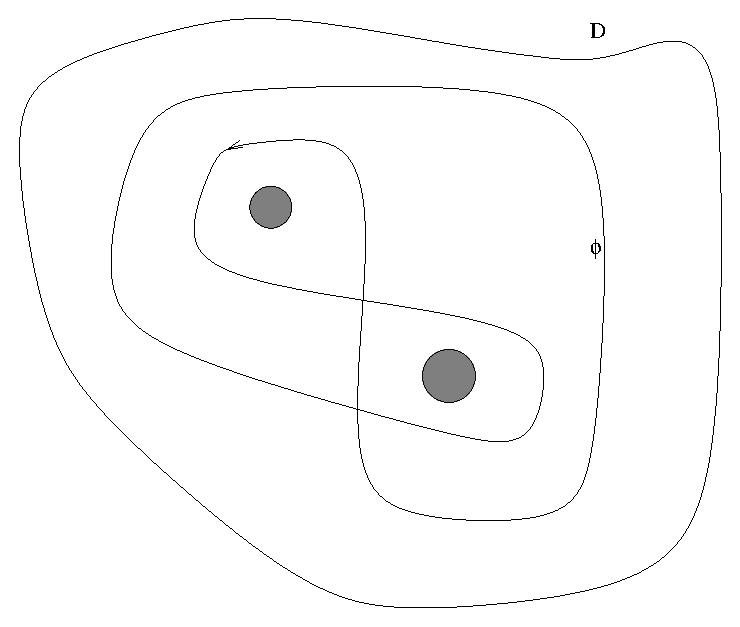
\includegraphics{homol.eps}}
\end{center}
\end{figure} 

Let $D$ be the domain and $\phi$ the path shown.  It can be shown by methods
of algebraic topology that $\phi$ is not contractible in $D$.  However, it
is also clear that $\int_\phi f(z) \ud z = 0$ for all analytic functions $f$ on
$D$. We shall ask which paths have this property.  This section of the course
is starred.

A chain\index{chain} in a domain $D$ is a finite sequence
$( \phi_1, \dots, \phi_N )$ of paths.  Two chains
$( \phi_1, \dots, \phi_N )$ and $( \psi_1, \dots, \psi_N )$ are directly
equivalent\index{directly equivalent} if there is a permutation $\pi$ of the
set $\{ 1, 2, \dots, N \}$ such that $\psi_i = \phi_{\pi(i)}$ for every $i$.  A
subdivision\index{chain!subdivision} of a chain
$( \phi_1, \dots, \phi_N )$ is a chain
\[
( \phi_{11}, \phi_{12}, \dots, \phi_{1 M_1}, \phi_{21}, \dots, \phi_{2 M_2},
\dots, \phi_{N 1}, \dots, \phi_{N M_N} )
\]
such that $\phi_i = \phi_{i 1} \vee \phi_{i 2} \vee \dots \vee \phi_{i M_i}$
for every $i$.  Two chains are equivalent\index{chain!equivalent} if they
have directly equivalent subdivisions.

A cycle\index{cycle} is a chain $( \phi_1, \dots, \phi_N )$ such that
each $\phi_i$ is a closed path\footnote{It is more usual to define a cycle to
be a chain equivalent to what I have called a cycle.}.  Two cycles 
$( \phi_1, \dots, \phi_N )$ and $( \psi_1, \dots, \psi_N )$ are homotopic %
\index{cycle!homotopic} if
$\phi_i$ is homotopic $\psi_i$ for every $i$.  Two cycles
$\Phi = ( \phi_1, \dots, \phi_N )$ and $\Psi = ( \psi_1, \dots, \psi_N )$ are
homologous\index{cycle!homology} if there is a sequence
$\Phi = \Phi_0, \Phi_1, \dots, \Phi_K = \Psi$ such that for every $i$,
$\Phi_{i-1}$ and $\Phi_i$ are either equivalent or homotopic.

If $\Phi = ( \phi_1, \dots, \phi_N )$ is a chain in a domain $D$ and
$f \colon D \mapsto \C$ is continuous, then $\int_\Phi f(z) \ud z$ is defined to
be $\sum_{i=1}^N \int_{\phi_i} f(z) \ud z$.  If $\Phi$ is also a cycle, and
$z_0 \in \C \setminus \Phi^*$, then the winding number of $\Phi$ about $z_0$
is defined to be
\[
w(\Phi,z_0) = \sum_{i=1}^N w(\phi_i,z_0) = \frac{1}{2 \pi \imath} \int_\Phi
\frac{\ud z}{z-z_0}.
\]

\begin{theorem}
Let $D$ be a domain and $\Phi$ be a cycle homologous in $D$ to a point.  Then
$\int_\Phi f(z) \ud z = 0$ for every analytic function $f \colon D \mapsto \C$.
\end{theorem}
 
\begin{proof}
Trivial consequence of homotopy invariance.
\end{proof}

This certainly deals with the path shown above.  The converse of this theorem
is also true, but somewhat harder to prove.  The main result of this
section is a characterization in terms of winding numbers of those cycles
for which the integral of any analytic function vanishes.

\begin{theorem}
Let $D$ be a domain and let $\Phi$ be a cycle in $D$ with $w(\Phi,z_0) =
0$ for every complex number $z_0 \notin D$.  Then $\int_\Phi f(z) \ud z = 0$ for
every analytic function $f \colon D \mapsto \C$.
\end{theorem}

The converse of this theorem is obvious, using the function $f(z) = 
(z-z_0)^{-1}$.  In order to prove this theorem we need another set of
definitions from algebraic topology and 3 easy lemmas.

Given a real number $\delta > 0$, we define $\Sigma(\delta)$ to be the set
of all squares $S \subset \C$ of the form
\[
\{ z \in \C : m\delta \le \Re z \le (m+1) \delta, n \delta \le \Im z \le
(n+1) \delta \}
\]
where $m$ and $n$ are integers.  Given such a square $S$, we denote by
$\partial S$ the boundary of $S$, oriented anticlockwise.  A square complex %
\index{square complex} of mesh $\delta$ is a subset
$\Sigma \subset \Sigma(\delta)$.  If $\Sigma = \{ S_1, \dots, S_N \}$ is a
square complex, then an edge of one of the $S_i$ is called internal if it is
shared by some other $S_j$, and is otherwise called external.  The boundary
$\partial \Sigma$ of $\Sigma$ is defined to be the chain of all external
edges of $\Sigma$ (with their directions coming from the orientations of the
relevant $\partial S_i$).  We write $\Sigma^*$ for the union of the squares
that make up $\Sigma$ (so that $\Sigma^* \subset \C$ and $\Sigma \subset
P[\C]$).

\begin{lemma}
Let $\Sigma$ be a square complex.  Then $\partial \Sigma$ is equivalent to a
cycle.
\end{lemma}

\begin{proof}
We can form a directed graph, where the vertices are all points of the form
$\delta(m + n \imath)$ and the edges are the external edges of $\Sigma$
(with their directions).  It does not take long to check that at any vertex
the number of edges going in equals the number of edges coming out.  Now start
at a vertex $v$ which has at least one vertex which has at least one edge
coming out of it, and move along edges in the forward direction for as long as
possible without repeating an edge.  As there are finitely many edges this
process must stop, and because of the condition just mentioned must stop at
$v$.  The result is a closed path.  If we remove this path, we obtain a
directed graph with fewer edges satisfying the same condition, so by induction
the result is proved.
\end{proof}

\begin{lemma}
Let $\Sigma = \{ S_1, \dots, S_N \}$ be a square complex and let $D$ be a
domain containing $\Sigma^*$.  Let $f \colon D \mapsto \C$ be continuous.  Then
$\int_{\partial \Sigma} f(z) \ud z = \sum_{i=1}^N \int_{\partial S_i} f(z) \ud z$.
\end{lemma}

\begin{proof}
The contributions to the right-hand side from integrals along internal edges
cancel, leaving only the integrals along external edges, which by definition
is the left-hand side.
\end{proof}

\begin{lemma}
Let $\Sigma = \{ S_1, \dots, S_N \}$ be a square complex and let
$z_0 \in \inter (\Sigma^*)$.  Let $f$ be a function analytic on a domain that
includes $\Sigma^*$.  Then $f(z_0) = \frac{1}{2 \pi \imath} \int_{\partial
\Sigma} \frac{f(z)}{z-z_0} \ud z$.
\end{lemma}

\begin{proof}
Firstly, suppose $z_0$ lies in the interior of $S_i$ for some $i$.  When
$j \neq i$, Cauchy's theorem implies that $\int_{\partial S_j} \frac{f(z)}
{z-z_0} \ud z$.  Also, $\partial S_i$ is homotopic to $C_\delta (z_0)$ for some
$\delta > 0$, so by Cauchy's integral formula $f(z_0) = \frac{1}{2 \pi \imath}
\int_{\partial S_i} \frac{f(z)}{z-z_0} \ud z$.  The result then follows from
above lemma.

Now if $z_0$ lies on an internal edge the result follows by continuity. 
\end{proof}

\begin{proof}[Proof of theorem]
Let $X \subset D$ be $\C \setminus \{ z : w(\Phi,z) = 0 \} = \{ z : w(\Phi,z)
\neq 0\} \cup \Phi^*$.  Since $w(\Phi,z)$ is continuous on the open set
$\C \setminus \Phi^*$, we see that $\{ z : w(\Phi,z) = 0 \}$ is open, so that
$X$ is closed.  Also, since $w(\Phi,z) = 0$ on the unbounded component of
$\C \setminus \Phi^*$, $X$ is bounded.  Thus $X$ is compact, from which it
follows that we can choose $\delta > 0$ such that $B_{2 \delta} (z) \subset D$
whenever $z \in X$.

Define a square complex $\Sigma$ of mesh $\delta$ by taking every square
$S \in \Sigma(\delta)$ such that $S \cap C \neq \emptyset$.  Note that
$S$ is included even if $S$ intersects $X$ only on the boundary - this is 
important.  It is clear that $X \subset \Sigma^*$, but we also have
$X \subset \inter \Sigma^*$ as the definition of $\Sigma$ does not allow
$z \in X$ to be on an external edge.  Also, by our choice of $\delta$, we
have $\Sigma^* \subset D$.

Hence, if $z \in \Phi^* \subset X$, above lemma gives that $f(z) = 
\frac{1}{2 \pi \imath} \int_{\partial \Sigma} \frac{f(w)}{w-z} \ud w$.  It follows
that
\begin{align*}
\int_\Phi f(z) \ud z &= \frac{1}{2 \pi \imath} \int_\Phi \int_{\partial \Sigma}
\frac{f(w)}{w-z} \ud w \ud z \\
&= \int_{\partial \Sigma} f(w) \frac{1}{2 \pi \imath} \int_\Phi
\frac{\ud z}{w-z} \ud w \\
&= - \int_{\partial \Sigma} f(w) w(\Phi,w) \ud w.
\end{align*}

The above change of integrals will not be justified, but we are talking about
continuous functions on closed, bounded subsets of $\R$, where the
justification is relatively easy.  Now since $X \cap \partial \Sigma =
\emptyset$, we have $w(\Phi,w) = 0$ for every $w \in \partial \Sigma$.  This
completes the proof.
\end{proof}

\backmatter

\begin{thebibliography}{9}

\bibitem{Jameson} G.J.O. Jameson, \emph{A First Course on Complex
    Functions}, Chapman and Hall, out of print.
  
  {\sffamily \small This is a good book for the second half of the
    course --- but probably not as good as Priestley.}

\bibitem{Priestley} H.A. Priestley, \emph{Introduction to Complex
    Analysis}, OUP, 1990.
  
  {\sffamily \small This book is highly recommended for the second
    half of the course. }

\bibitem{Sutherland} W.A. Sutherland, \emph{Introduction to Metric and
    Topological Spaces}, OUP, 1975.

  {\sffamily \small This book is quite good for the first half of the
    course. }

\end{thebibliography}

There are a lot of books on this course.  Quality is variable.

\printindex
\end{document}
